%% LyX 2.0.1 created this file.  For more info, see http://www.lyx.org/.
%% Do not edit unless you really know what you are doing.
\documentclass[letterpaper, 10 pt, conference]{ieeeconf} 

\IEEEoverridecommandlockouts

\overrideIEEEmargins 

\usepackage[T1]{fontenc}
\usepackage[latin9]{inputenc}
\usepackage{amstext}
\usepackage{graphicx}
\usepackage{esint}

\makeatletter

%%%%%%%%%%%%%%%%%%%%%%%%%%%%%% LyX specific LaTeX commands.
\newcommand{\noun}[1]{\textsc{#1}}
%% Because html converters don't know tabularnewline
\providecommand{\tabularnewline}{\\}

%%%%%%%%%%%%%%%%%%%%%%%%%%%%%% User specified LaTeX commands.
\renewcommand{\b}[1]{\mbox{\boldmath$#1$}}
\let\vec\b

\makeatother

\usepackage[english]{babel}
\begin{document}

\title{\LARGE \bf Predicting Object Interactions from Contact Distributions}


\author{Oliver Kroemer$^{1}$ and Jan Peters$^{1,2}$}


\thanks{$^{1}$Oliver Kroemer and Jan Peters are with the Intelligent Autonomous Systems group at the Technische Universitaet Darmstadt, Germany. \newline $^{2}$ Jan Peters is also with the Max Planck Institute for Intelligent Systems.
 {\tt\small  \{kroemer,peters\}@ias.tu-darmstadt.de}
}




\maketitle
\begin{abstract}
Contacts between objects play an important role in manipulation tasks.
Depending on the locations of contacts, different manipulations or
interactions can be performed with the object. By observing the contacts
between two objects, a robot can learn to detect potential interactions
between them. 

Rather than defining a set of features for modeling the contact distributions,
we propose a kernel-based approach. The contact points are first
modeled using a Gaussian distribution. The similarity between these
distributions is computed using a kernel function. The contact distributions
are then classified using kernel logistic regression. The proposed
approach was used to predict stable grasps of an elongated object,
as well as to construct towers out of assorted toy blocks. 
\end{abstract}

\section{Introduction}

Manipulation tasks almost always involve direct physical contact between
two or more objects. These contacts can be between different objects
in the robot's environment, or between an object and the robot. Depending
on the locations of the contacts, different types of interactions
and manipulations can occur. For example, a contact on the side of
an object may allow for pushing and sliding the object, while a contact
on the bottom can be used for lifting or supporting the object. In
order to successfully perform a manipulation task, a robot must be
able to determine the potential interactions between objects and utilize them
to accomplish the task's goal. 

Utilizing contact information in an efficient manner is however not
a trivial task. Analytical approaches tend to require accurate models
of the objects, and rely on simplified contact models \cite{GraspSurveyBohg}.
In an effort to make robots more autonomous, learning approaches have
become more widely adopted in the field of robot manipulation \cite{objectPlacementYun,KopickiZSMW11,SimulatedAffordanceLearning}.
However, representing contacts between objects often relies on hand-crafted
features for the given task. 

In this paper, we propose an example-based learning approach to detect
interactions between objects from their contact distributions. We
pose the problem of detecting interactions as a binary classification
problem, wherein the robot has to predict whether or not a certain
interaction is occurring based on the geometry and relative poses
of the objects. The robot first computes which regions of the objects
are in contact with each other. The resulting cloud of contact points
is subsequently modeled as a Gaussian distribution. A Bhattacharyya
kernel function \cite{JebaraK03} can then be used to compute the
similarities between the contact distributions and, thus, classify
them using kernel logistic regression. In this manner, the robot uses
the similarity between the current contact distribution and previous
distributions in order to classify the potential interaction. The
details of the approach are explained in Section \ref{sec:Classifying-Object-Interactions}.

The proposed approach was implemented on the real robot shown in Fig.
\ref{fig:The-Darias-robot}. In the first experiment, the robot was
given the task of predicting which grasps allow it to steadily pick
up an elongated object. The second experiment required the robot to
stack assorted blocks. The details of the experiments are given in
Section \ref{sec:Experiments}.
\begin{figure}
\begin{centering}
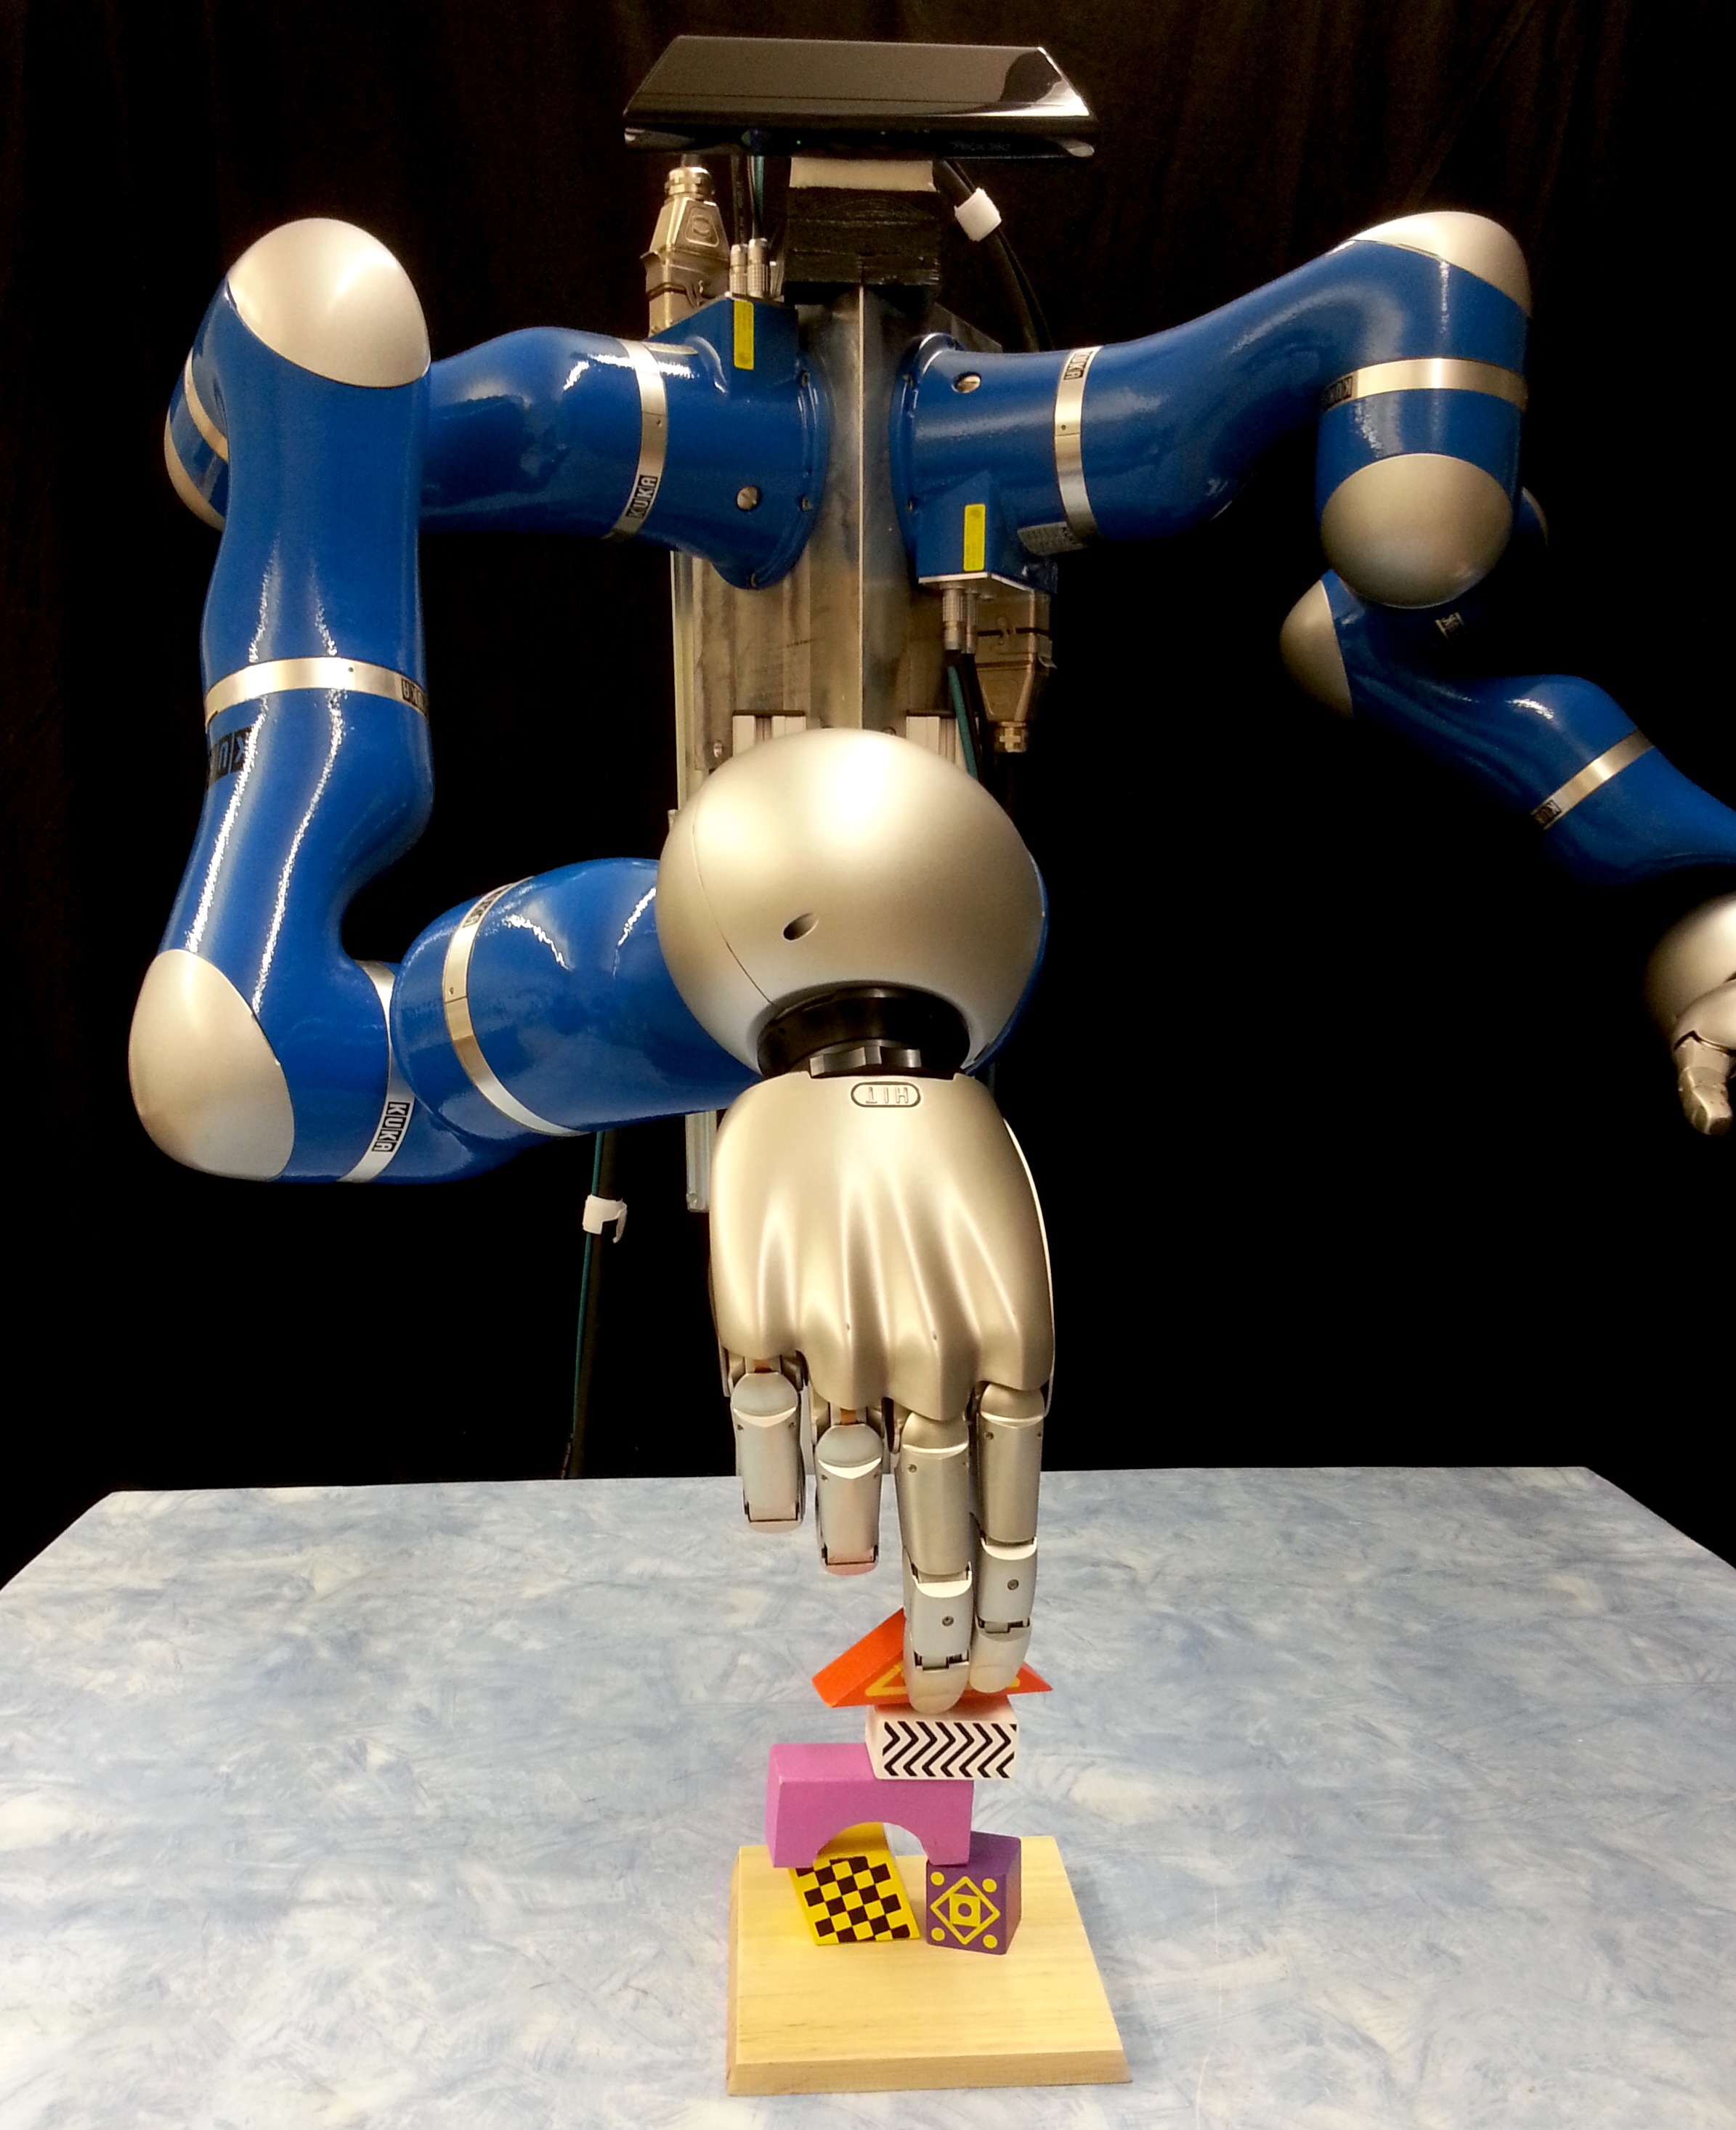
\includegraphics[width=0.89\columnwidth]{PicsforIROS2014/RobotStacking}
\par\end{centering}

\caption{\label{fig:The-Darias-robot}The Darias robot performing a block stacking
task.}
\end{figure}



\section{Learning From Contact Distributions\label{sec:Classifying-Object-Interactions}}

In this section, we first outline related work in interaction detection.
In Sections \ref{sub:Contact-Points} to \ref{sub:Computing-Contact-Distributions},
we explain how contacts between objects are detected and used to create
contact distributions. In Sections \ref{sub:Comparing-Contact-Distributions}
to \ref{sub:Classifying-Contact-Distribution}, we provide a kernel
function for computing the similarity between contact distributions
and explain how it is used to classify the distributions using kernel
logistic regression. 


\subsection{Related Work}

\begin{figure}
\begin{centering}
\begin{tabular}{cc}
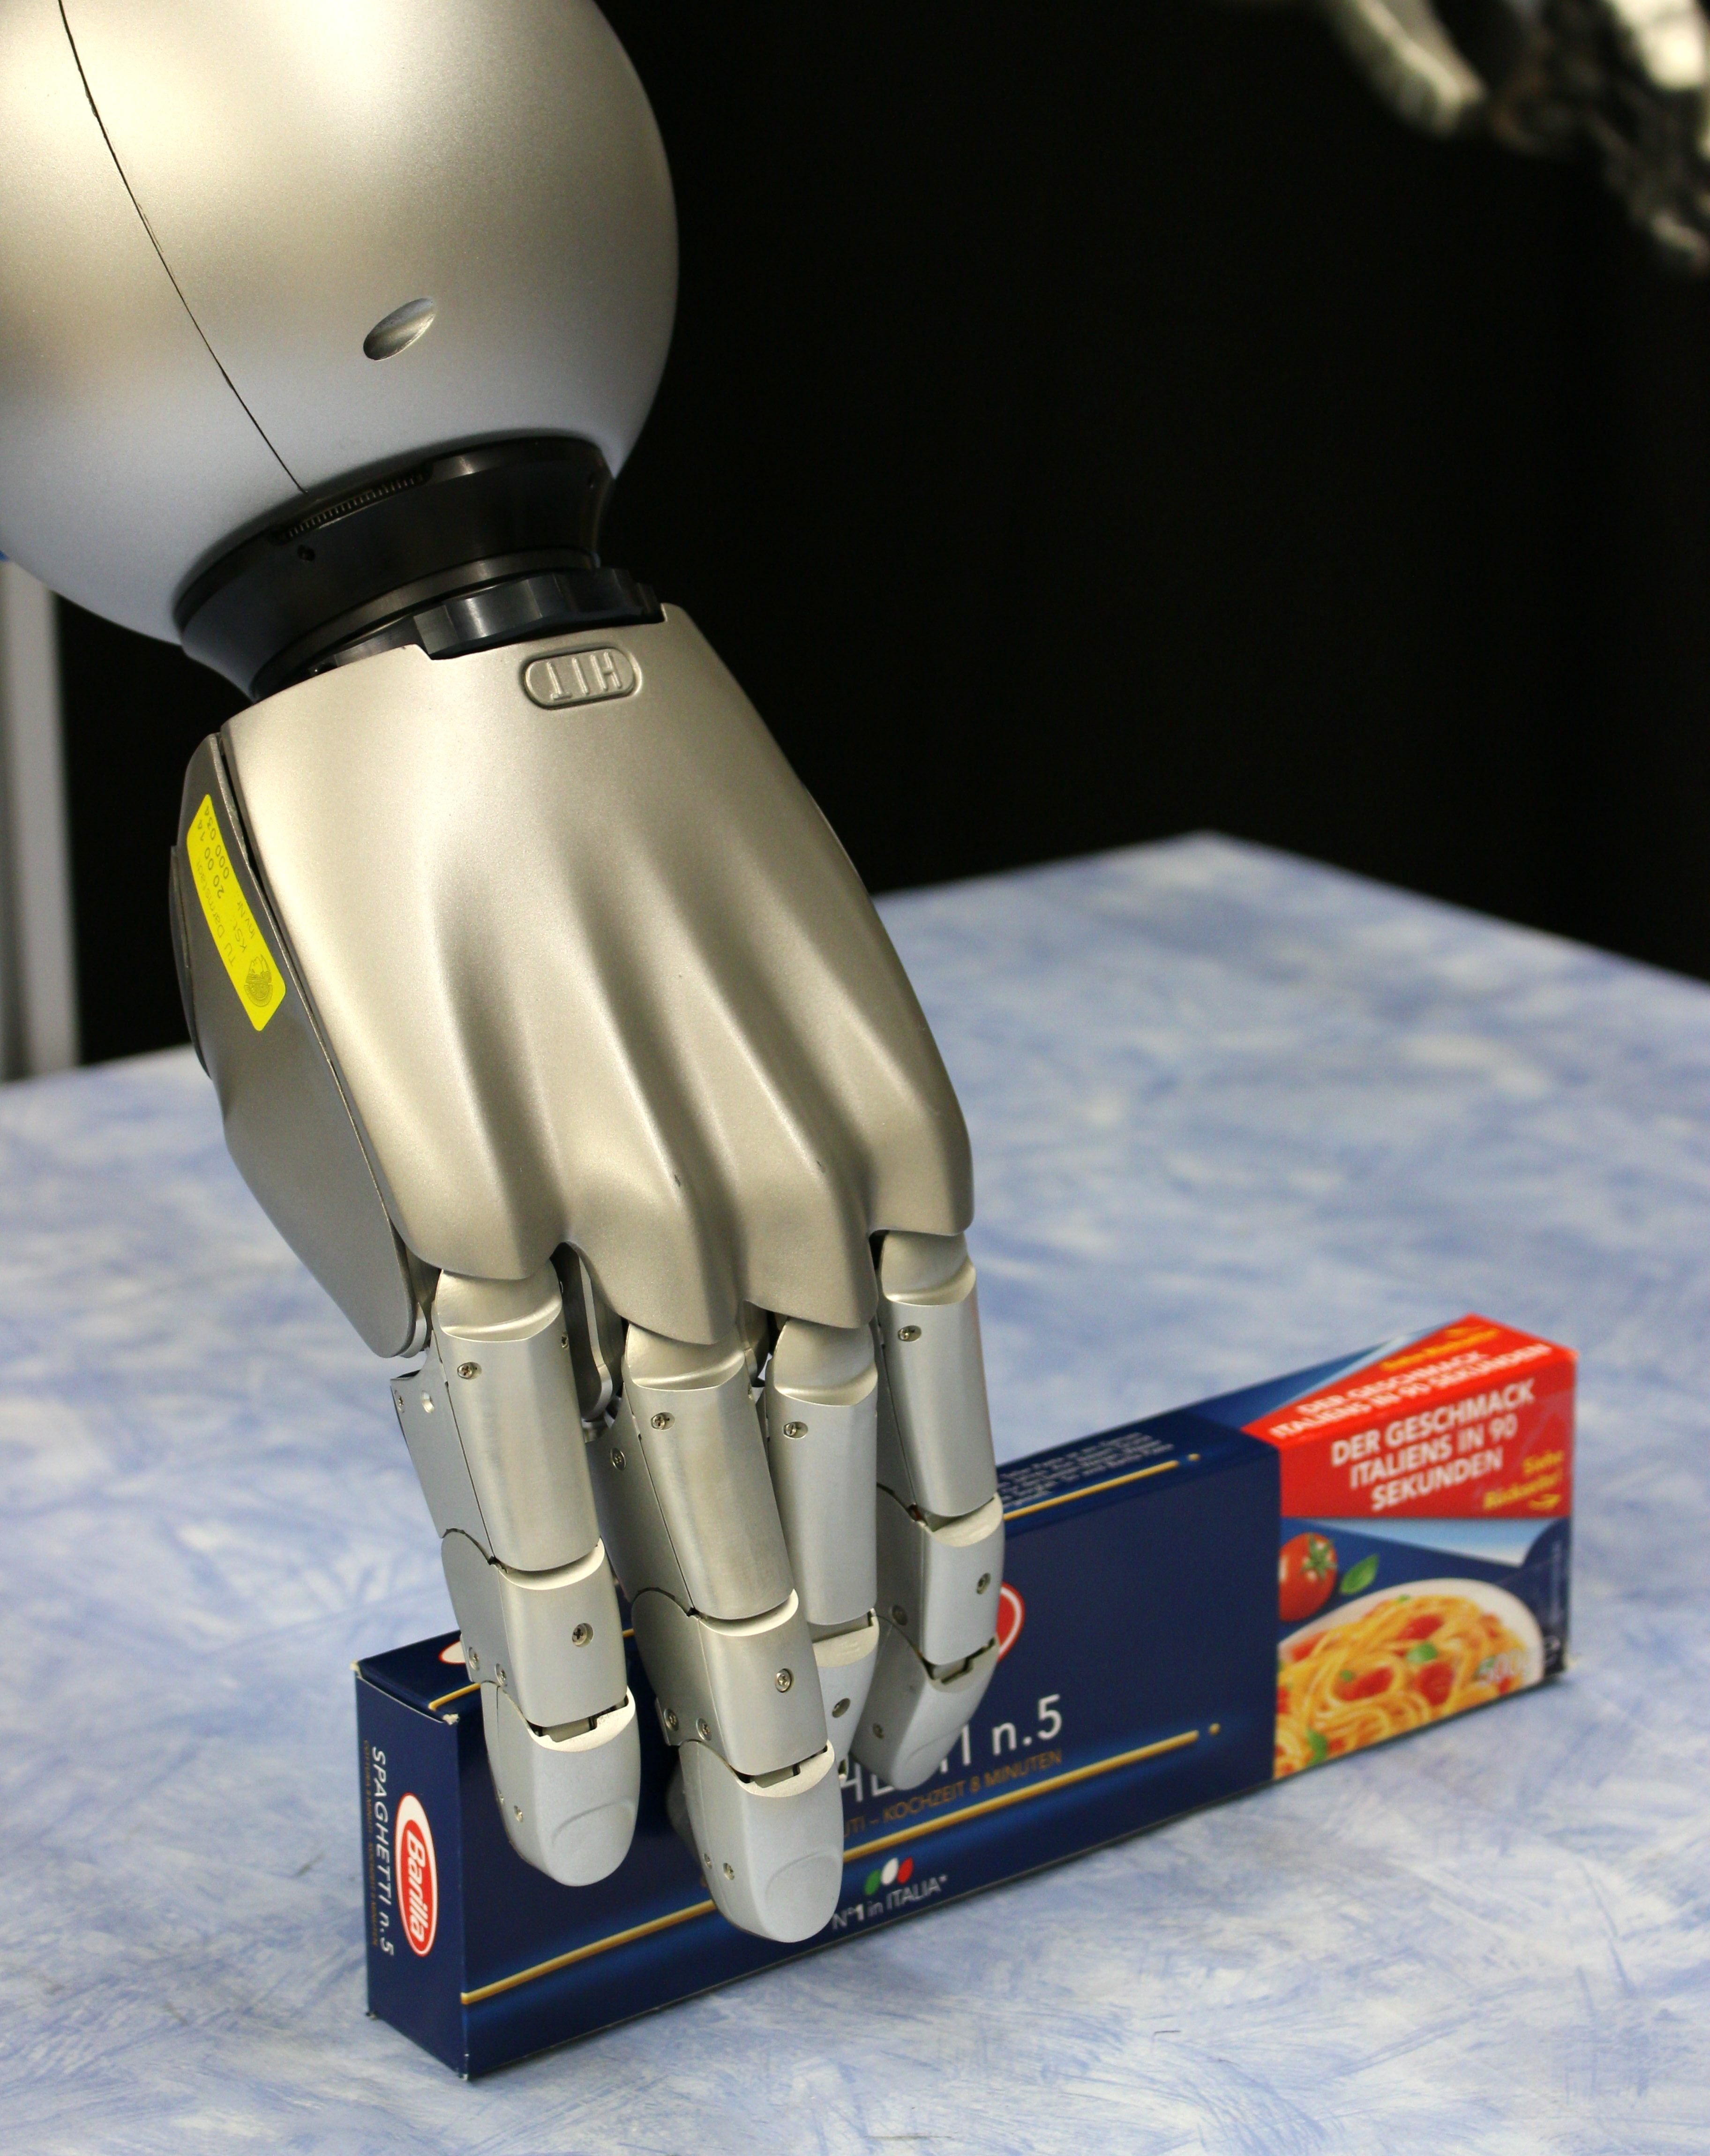
\includegraphics[width=0.46\columnwidth]{PicsforIROS2014/3FingGrasp} & 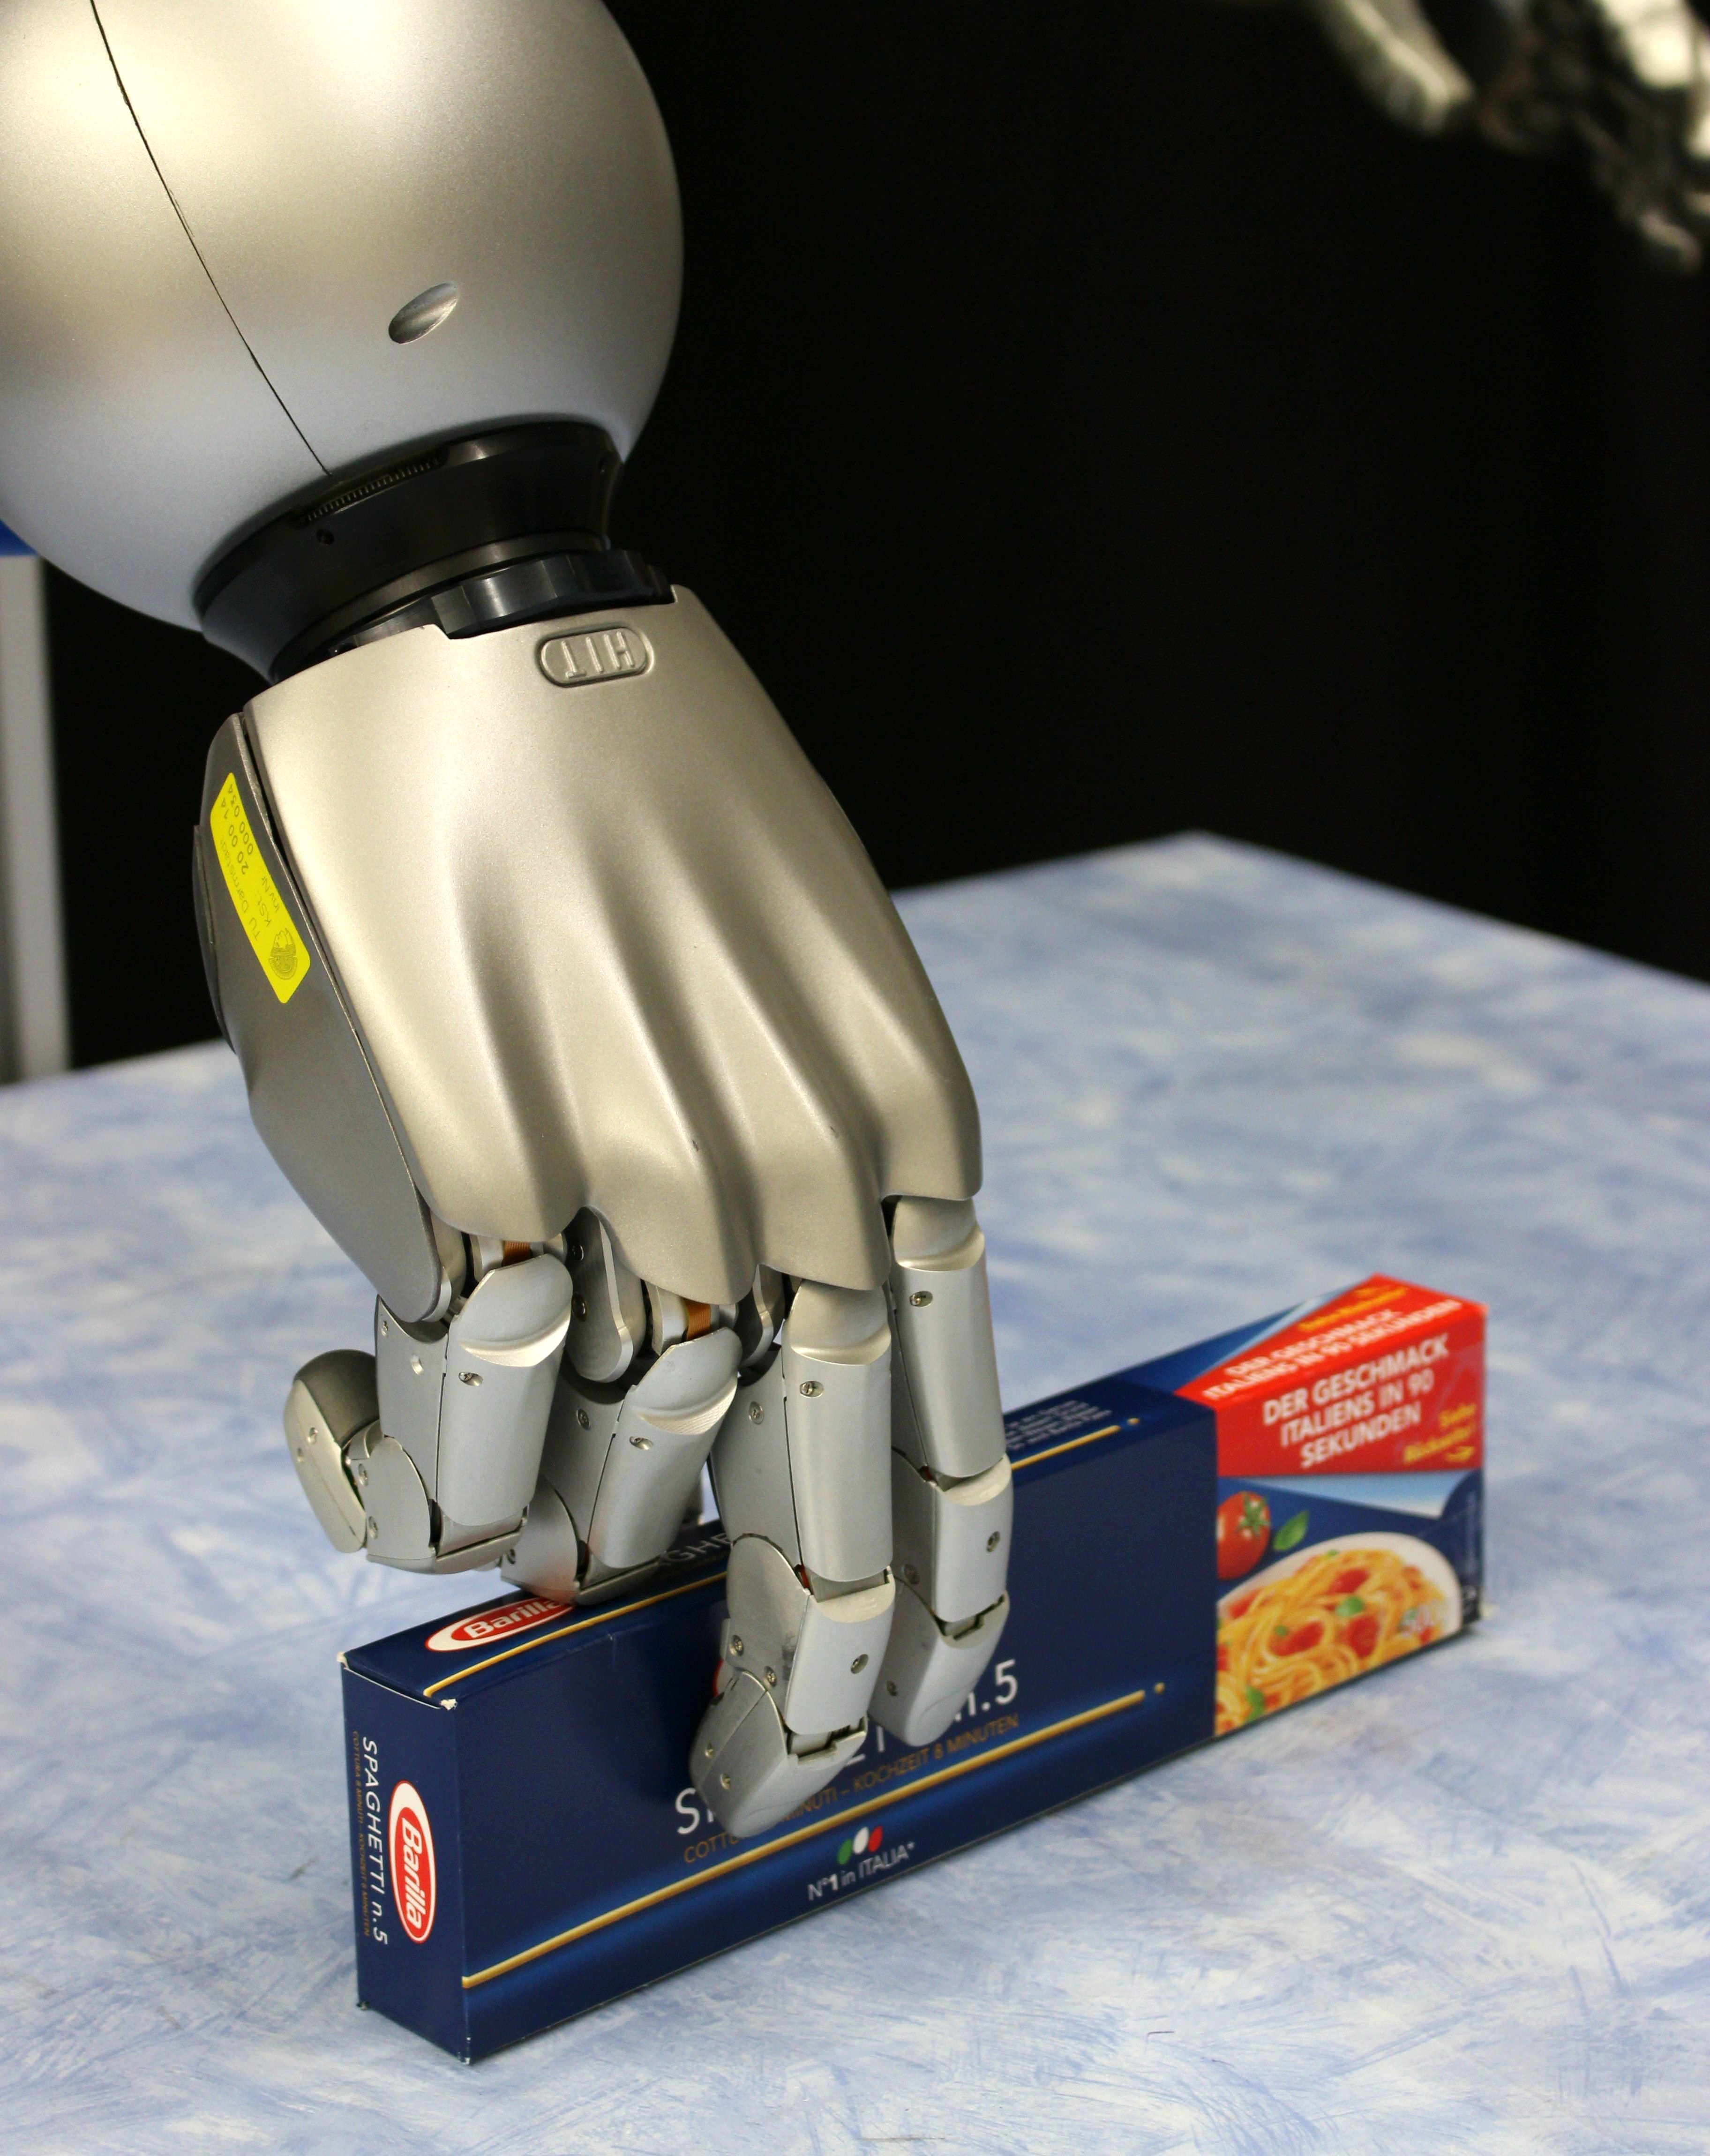
\includegraphics[width=0.46\columnwidth]{PicsforIROS2014/4FingGrasp}\tabularnewline
3-Fingered Grasp & 4-Fingered Grasp\tabularnewline
\end{tabular}
\par\end{centering}

\caption{\label{fig:Grasp-types}The two types of grasps that were used during
the lifting experiment. The three-fingered grasp uses the tips of
the thumb, middle, and index fingers in order to pinch the object. The ring and little finger are not touching the box.
The four-fingered grasp additionally uses the back of the ring finger
on the top of the box in order to provide additional support. }
\end{figure}
Learning symbolic representations of geometric relations between objects,
e.g. object A is \noun{on} object B, is an important skill for performing
complex manipulation tasks. Rosman and Ramamoorthy \cite{ContactNetwork}
proposed the use of a contact network to learn the spatial relations
between objects. Contact points were detected using a support vector
machine to separate the point clouds of the objects. The vectors between
the objects' contact points were then computed and used to classify
relations such as \emph{on} and \emph{adjacent} using a $k$-nearest
neighbors classifier. Kulick et al. use an active learning approach
to efficiently learn a symbolic representation of the relations between
objects \cite{kulickSymbolLearning}. Using features such as the heights
of objects and the relative positions between objects, they train
a Gaussian process classifier to learn in which geometric states the
predicate is true. 

Classifying interactions between objects is also closely related to
learning affordances \cite{gibson1979}. If an object allows a robot
to perform an action with it, than the object is said to ``afford''
that action. Affordances have been widely studied in robotics \cite{ToAffordorNottoAfford,koppula2013_anticipatingactivities,MontesanoBayesNetAffordance},
and especially in the field of robot grasp synthesis \cite{GraspSurveyBohg}.
Recently, several papers have proposed template-based approaches for
detecting where an object can be grasped \cite{Herzog_AR_2013,detry2012a,Kroemer_ICRA_2012}.
These approaches predict where to grasp an object based on the local
shape of the object relative to the hand. The approach presented by
Detry et al. \cite{detry2012a} learns both the bounding box of points
to consider when comparing grasps as well as a dictionary of graspable
parts. 

Contact information can also be represented in the form of tactile
sensor readings. Bekiroglu et al. \cite{bekiroglu2011d} proposed
learning to predict stable grasps of objects using kernel logistic
regression. Their approach used a product of three separate kernels
based on the position of the hand relative to the object, the approach
direction of the hand, and moment features of the tactile sensor arrays'
readings. In the work of Dang et al. \cite{DangA12Bag-of-features},
the locations of the sensed contact points are defined relative to
the palm, and modeled using a bag-of-words representation. A support
vector machine is then trained to classify stable and unstable grasps.

The features used by learning algorithms can also be designed to capture
specific aspects of the contacts between objects. In \cite{SimulatedAffordanceLearning},
a classifier was trained on simulated data to predict interactions,
such as support and location control, between pairs of objects. The
classifier was provided with 93 features, such as the total contact
patch area, and the vector between the closest contact point and the
other object. Automatic relevance determination was then used to effectively
select a subset of these features. Jiang et al. \cite{objectPlacementYun}
addressed the problem of learning to place objects in a scene. The
placement of an object was represented by a set of $145$ features,
including features for modeling supporting contacts and the caging
of objects. A support vector machine with a shared sparsity structure
was then used to classify good and bad placements of objects. 


\subsection{Contact Points\label{sub:Contact-Points}}

\begin{figure}
\begin{centering}
\begin{tabular}{cc}
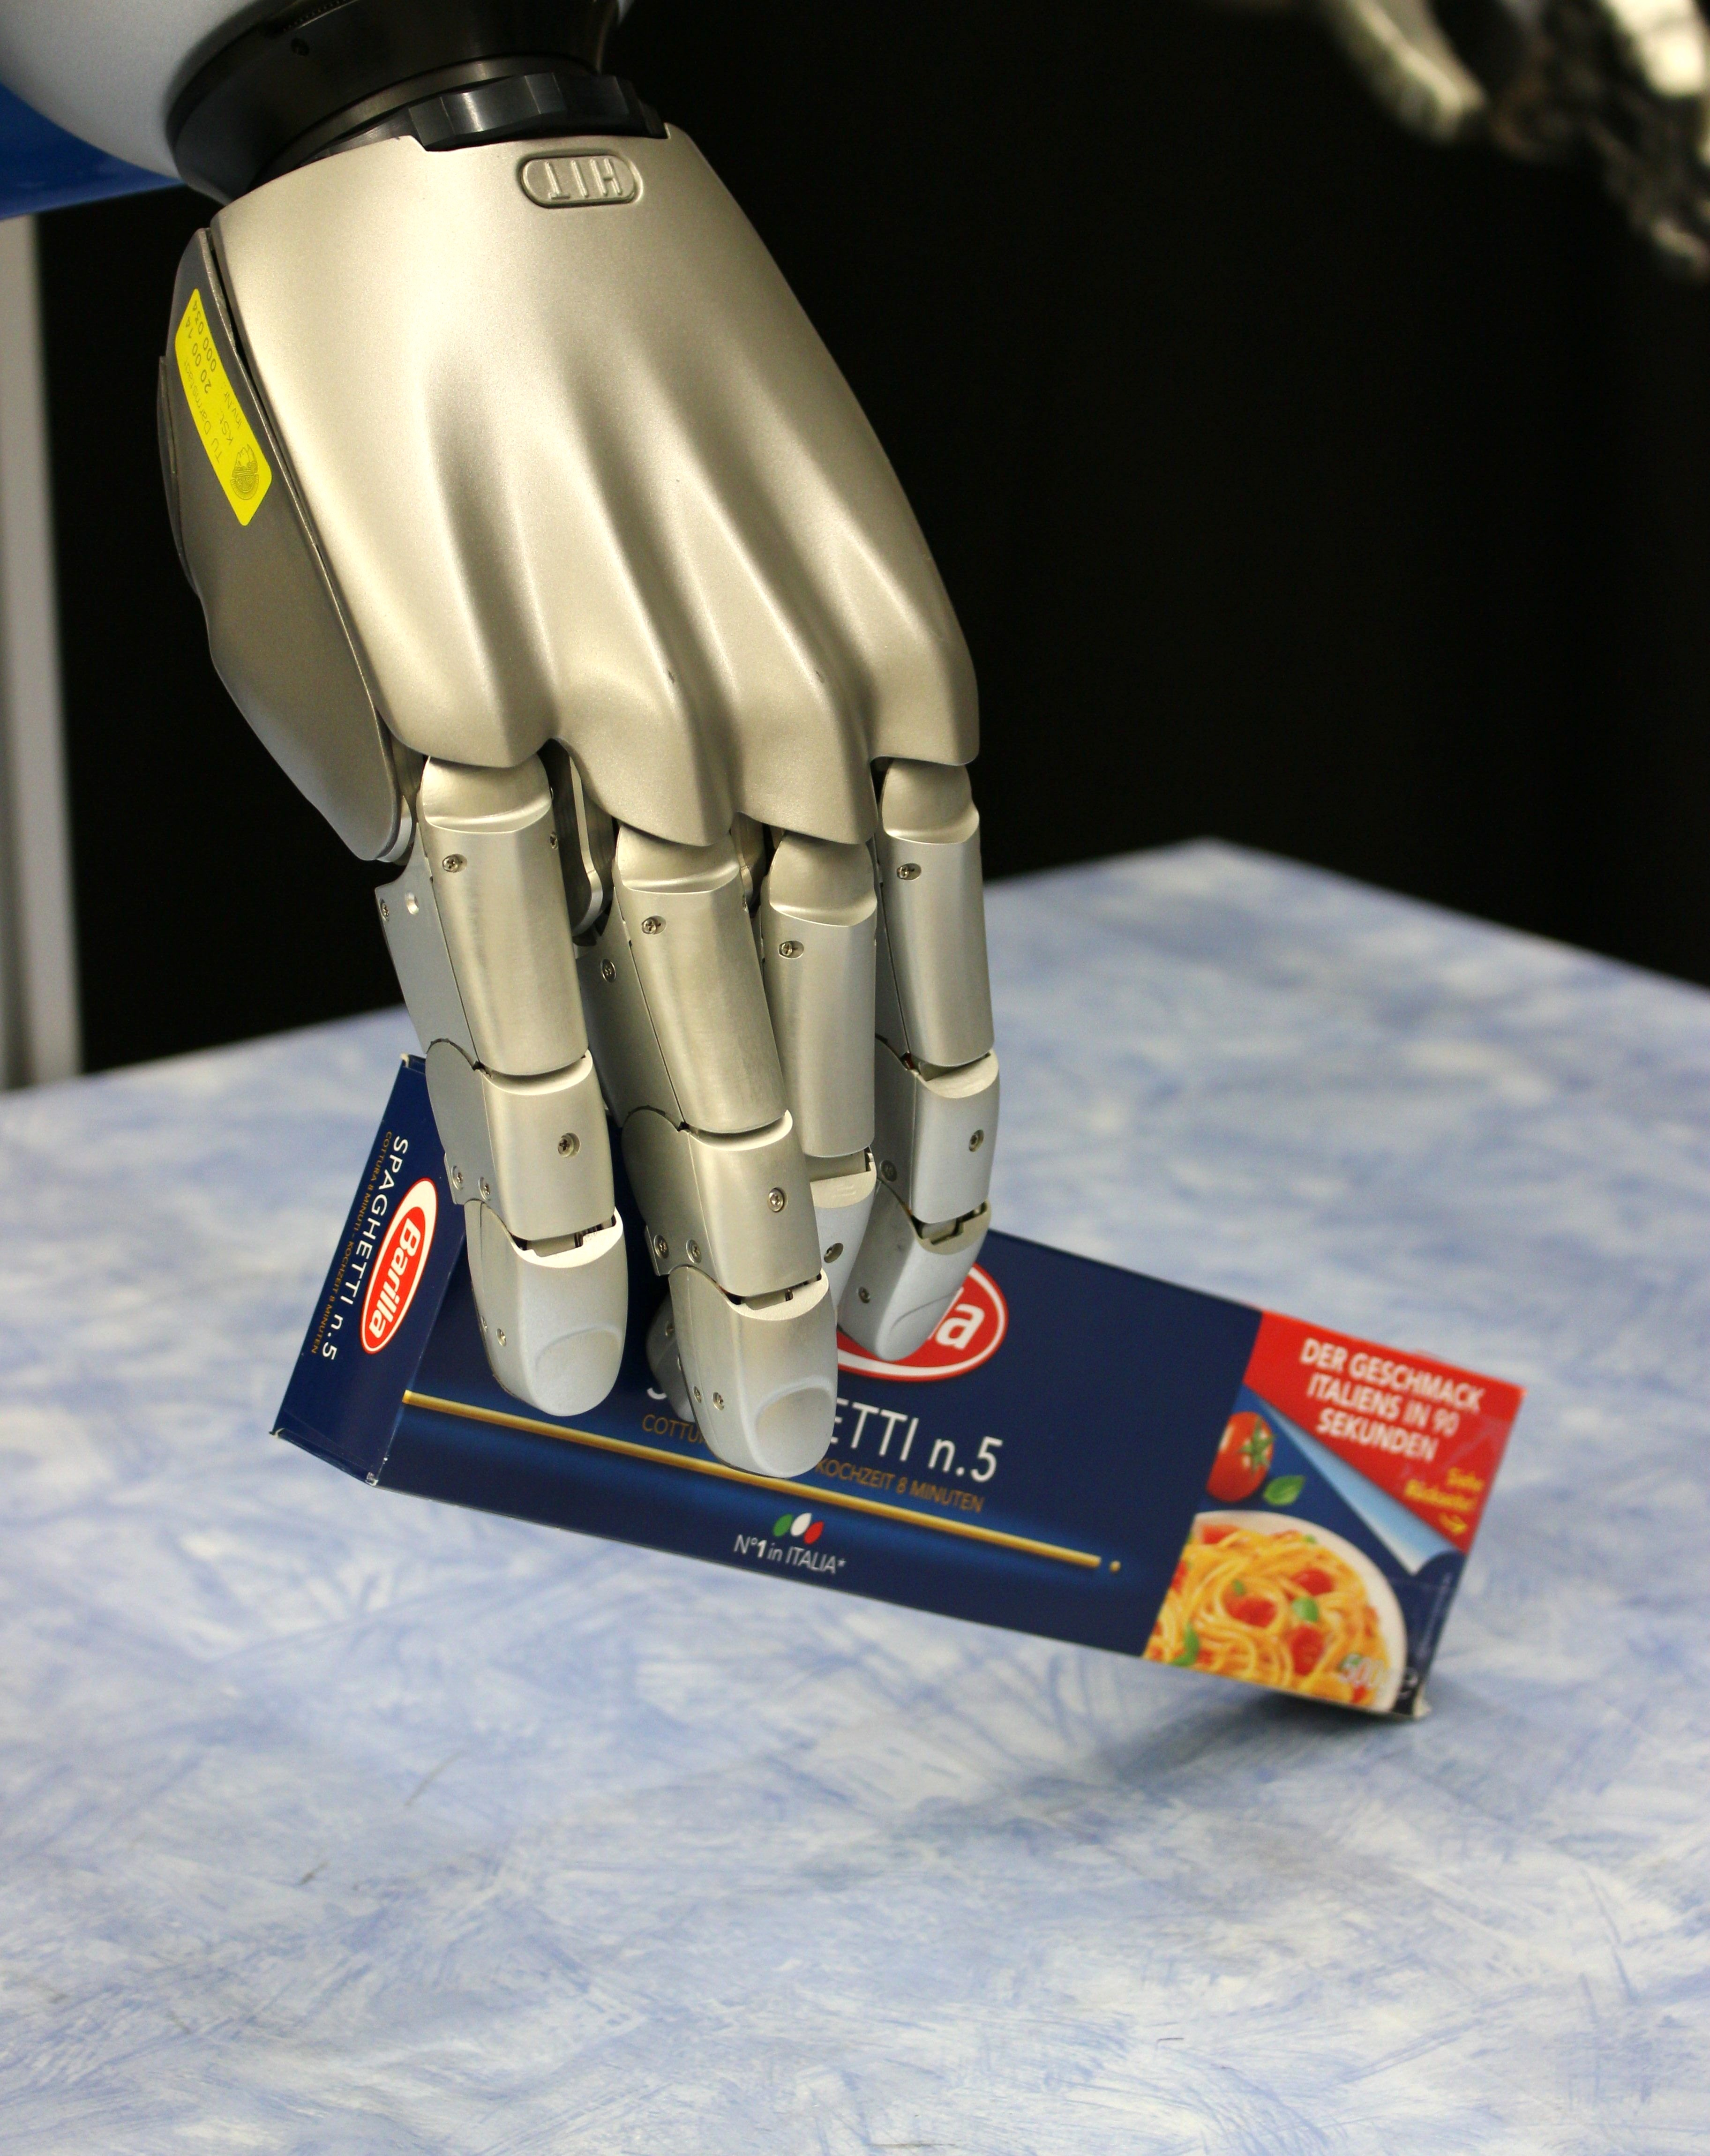
\includegraphics[width=0.46\columnwidth]{PicsforIROS2014/3FingLift} & 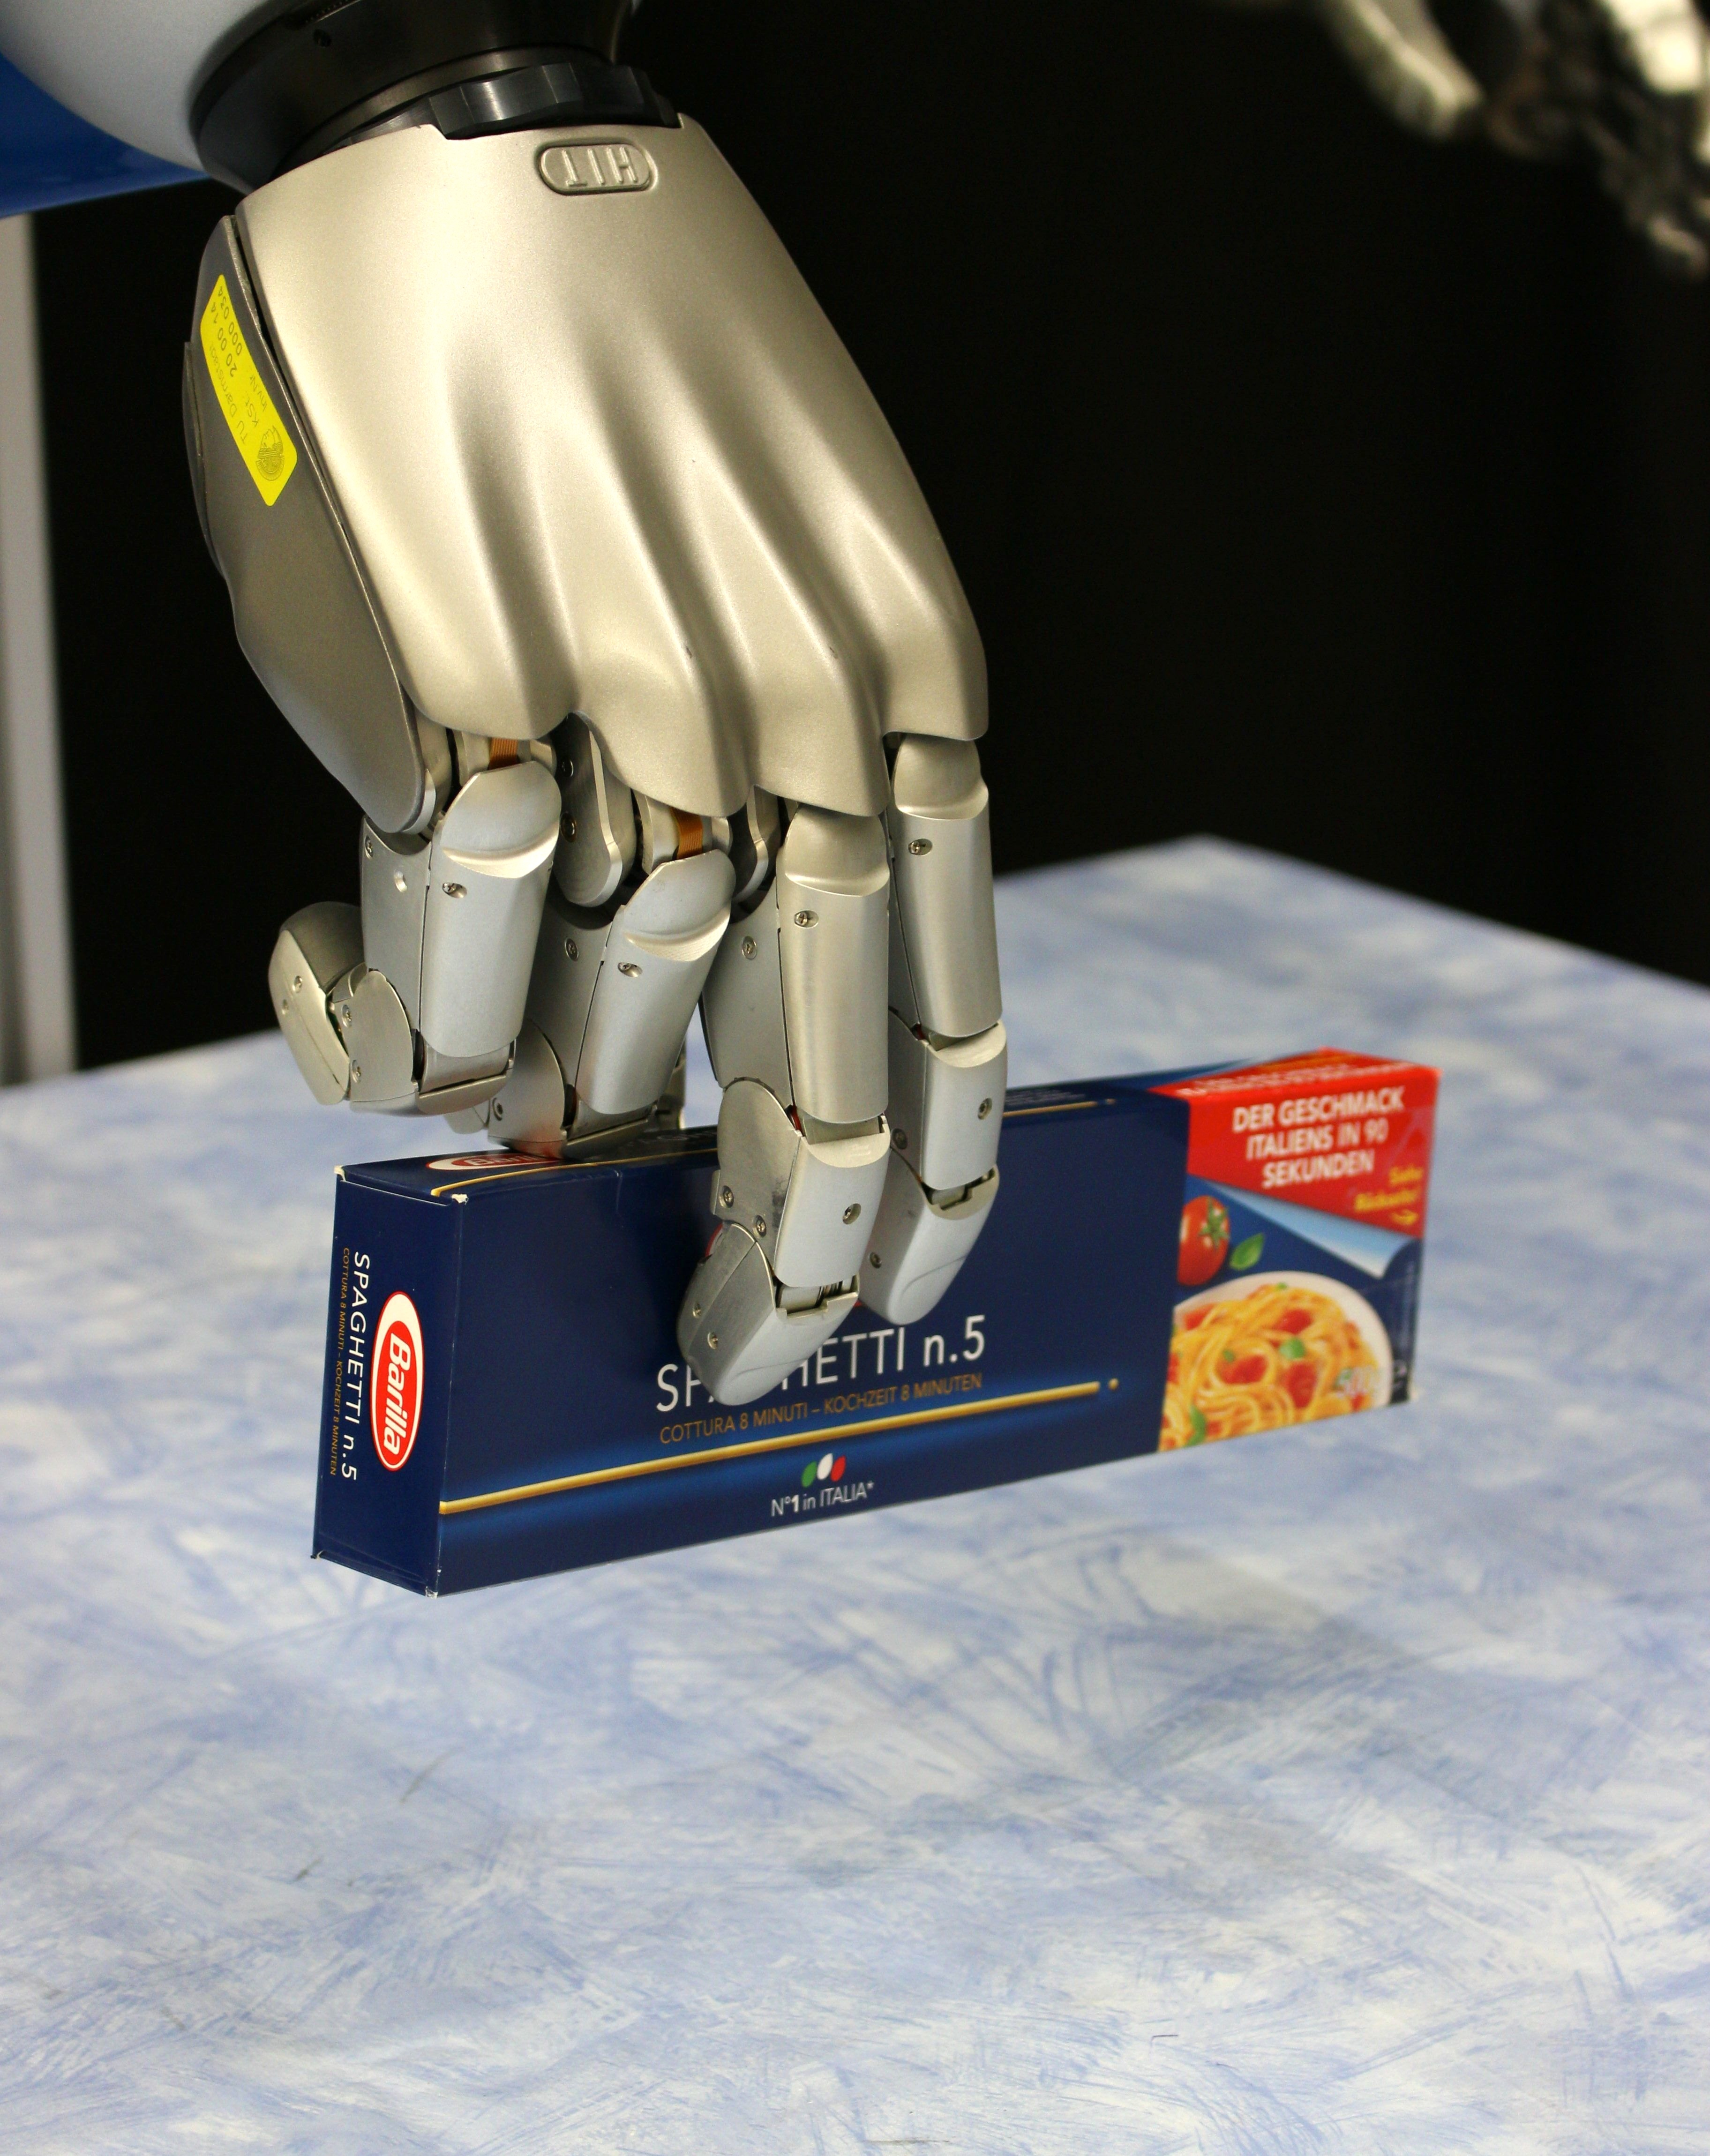
\includegraphics[width=0.46\columnwidth]{PicsforIROS2014/4FingLift}\tabularnewline
Failed Lift & Successful Lift\tabularnewline
\end{tabular}
\par\end{centering}

\caption{\label{fig:good-and-bad-lift}Examples of failed and successful lifts.
A lift was considered a failure if the object was still touching the
table at the end of the trial.}
\end{figure}
In order to determine the contacts between objects, we first need
a suitable representation of the object and its geometry. Given an
object $O_{i}$, where $i$ specifies the index of the object, we
define its geometry as a point cloud with $n_{i}$ points at positions
$\vec{p}_{ij}$ and corresponding normals $\vec{u}_{ij}$ for $j\in\{1,\ldots,n_{i}\}$.
Point clouds are flexible object representations that are widely used
in robotics \cite{Rusu_ICRA2011_PCL}. The normals of the points are
straightforward to compute using the covariance of nearby points and
the viewing direction.

The point cloud defines the surface of the object and, hence, also
where contacts can potentially be made with another object. In order
to obtain a set of contact points, each point in the point cloud is
classified as either being in contact with the other object or not.
In our experiments, we used logistic regression to classify the points, although 
other methods for detecting contacts are also applicable.
The probability of a point $\vec{p}_{ic}$ being in contact with the
object $O_{j}$ is given by 
\[
p(\text{contact}|\vec{p}_{ic},\vec{u}_{ic},O_{j})=\left(1+\exp\left(\vec{\phi}^{T}\vec{\rho}\right)\right)^{-1},
\]
where $\vec{\phi}$ is a vector of feature functions and $\vec{\rho}$
is a vector of corresponding weights. We used three features, including
a density estimation
\[
\phi_{1}(\vec{p}_{ic},O_{j})=\sum_{k}\exp\left(-\frac{\left\Vert \vec{p}_{ic}-\vec{p}_{jk}\right\Vert ^{2}}{\sigma^{2}}\right)
\]
and a surface normal density estimation 
\[
\phi_{2}(\vec{p}_{ic},\vec{u}_{ic},O_{j})=\sum_{k}(\vec{u}_{ic}^{T}\vec{u}_{jk})\exp\left(-\frac{\left\Vert \vec{p}_{ic}-\vec{p}_{jk}\right\Vert ^{2}}{\sigma^{2}}\right)
\]
where $\sigma$ is the length scale of the density. We also include
a bias term $\phi_{3}=1$. 

These three features are well-suited for detecting arbitrary contacts between two objects.
Some interactions however require specific types of contacts, e.g., cutting requires contact with a sharp edge. The set of features can be easily extended for more specific types of contacts. 



Computing a set of weights $\vec{\rho}$
that maximizes the likelihood of the training data is a convex optimization
problem, and can be solved using iterative reweighted least squares,
as explained in \cite{Bishop}. A point is classified as a contact
point if the probability of contact is greater than $0.5$. 
\begin{figure*}
\begin{centering}
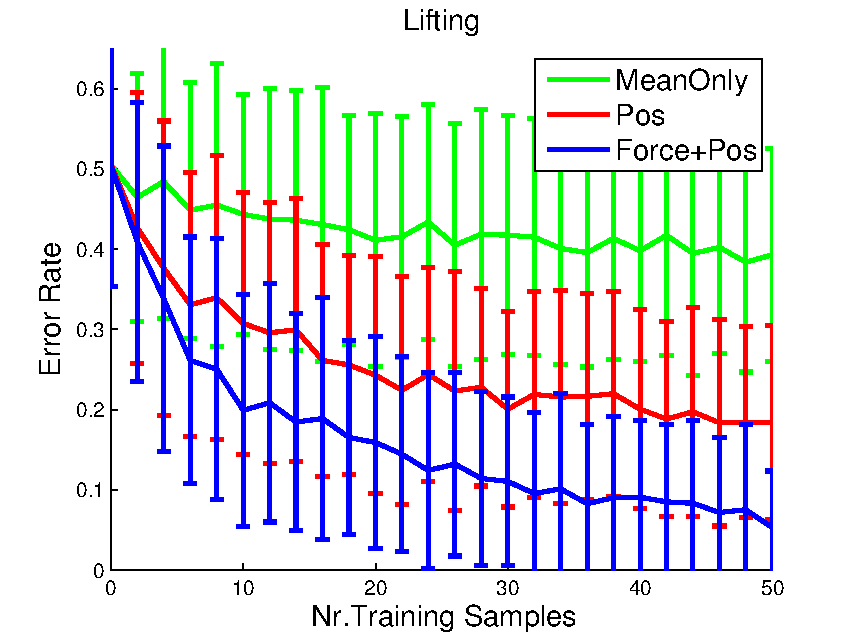
\includegraphics[width=0.47\linewidth]{PicsforIROS2014/LiftResultsA}\hspace{5mm}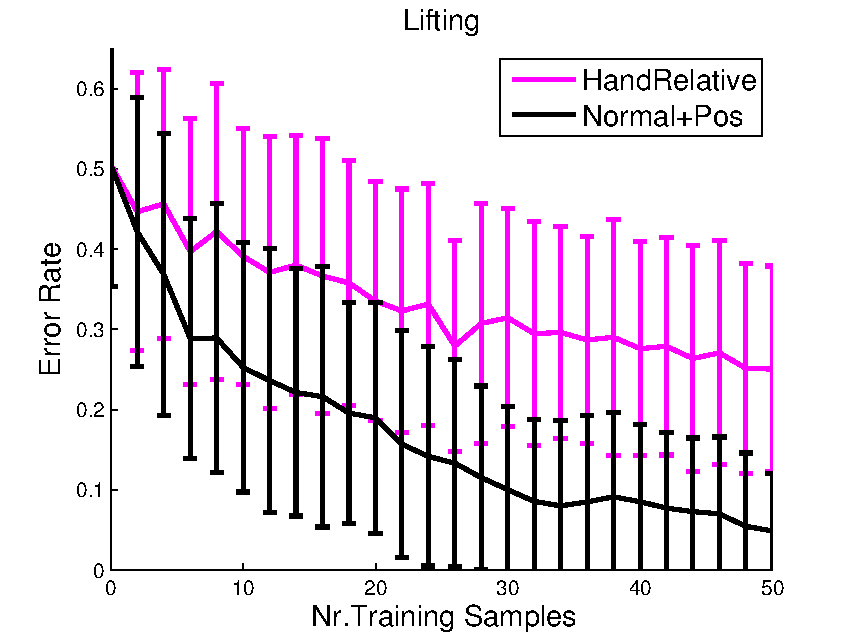
\includegraphics[width=0.47\linewidth]{PicsforIROS2014/LiftResultsB}
\par\end{centering}

\caption{\label{fig:Lifting-Results}The expected error rates for the lifting
task. The error bars indicate one standard deviation. An error rate
of $1$ indicates that none of the test samples were correctly classified,
and an error rate of $0$ is achieved when the classifier evaluates
all of the samples correctly.}
\end{figure*}



\subsection{Object Centers\label{sub:Object-Centers}}

In addition to the shape of the object, we also define a set of \emph{object
centers} for each object. Object centers are used to define interaction-relevant
coordinate frames for the object. Each center $\vec{c}_{ik}$, where
$k$ is the index of the center for object $O_{i}$, is associated
with a position $\vec{x}_{ik}$ and at least one axis $\vec{a}_{ik}$.
For example, the position of an object's center of gravity is given
by the mean point of its mass, and an axis pointing down in the direction
of gravity. For an articulated object, such as a hand winch or door
handle, the position and axis of rotation of the revolute joint defines
another center. Although an object may have many centers, usually
only one center is used for predicting an interaction. In this paper,
we only consider a single object center $\vec{c}_{i}$, and leave
automatically selecting the relevant center to future work.

Once the contact points have been found, they need to be defined with
respect to the center's coordinate frame. If the axes of the center
already defines three orthogonal axes $\vec{a}_{i}^{x}$, $\vec{a}_{i}^{y}$,
and $\vec{a}_{i}^{z}$ this step is trivial. However, the center of
gravity or the center of a revolute joint only define a single axis
$\vec{a}_{i}^{x}$ and not a full 3D coordinate frame. In order to
define the other two axes, we first project the contact points into
a 2D plane, with the normal of the plane given by the first axis of
the center $\vec{a}_{i}^{x}$. We then compute the matrix of second moments
 about the center position for the contact points, and subsequently compute the eigenvectors
of the matrix. The second axis $\vec{a}_{i}^{y}$ is defined by the
eigenvector with the largest eigenvalue, such that the mean of the
contact points is in the positive direction. Using this approach,
the contact point clouds are aligned according to the radial direction
with the largest variance. The third axis is simply given by the cross
product of the first two $\vec{a}_{i}^{z}=\vec{a}_{i}^{x}\times\vec{a}_{i}^{y}$. 

The positions of the $\tilde{n}_{i}$ contact points in the object
center's coordinate frame are denoted as $\tilde{\vec{p}}_{ij}$ with
corresponding normals $\tilde{\vec{u}}_{ij}$ for $j\in\{1,\ldots,\tilde{n}_{i}\}$. 


\subsection{Computing Contact Distributions\label{sub:Computing-Contact-Distributions}}

Having computed a set of contact points, we now want to compare this
set of contacts to previously observed ones. Rather than comparing
points individually, we first model the set of contact points as a
distribution. In particular, we model them as a 6D Gaussian distribution,
where the first three dimensions correspond to the positions of points,
and the last three model the normals. In the lifting experiment in
Section \ref{sec:Experiments}, we also investigate replacing the
normals of each point with an estimate of the force. However, the
forces are in most cases not known, especially when the interaction
is between two objects and not with the robot.

Given a set of contacts, we now define a distribution over contact
points as a Gaussian distribution. The mean vector $\vec{\mu}_{i}$
and variance $\vec{\Sigma}_{i}$ of the distribution are given as
\[
\vec{\mu}_{i}=\frac{1}{\tilde{n}_{i}}\sum_{k=1}^{\tilde{n}_{i}}\left[\begin{array}{c}
\tilde{\vec{p}}_{ik}\\
\tilde{\vec{u}}_{ik}
\end{array}\right],
\]
\[
\vec{\Sigma}_{i}=\frac{1}{\tilde{n}_{i}}\sum_{k=1}^{\tilde{n}_{i}}\left(\left[\begin{array}{c}
\tilde{\vec{p}}_{ik}\\
\tilde{\vec{u}}_{ik}
\end{array}\right]-\vec{\mu}_{i}\right)\left(\left[\begin{array}{c}
\tilde{\vec{p}}_{ik}\\
\tilde{\vec{u}}_{ik}
\end{array}\right]-\vec{\mu}_{i}\right)^{T}.
\]
This model provides a compact representation of the mean contact position
and normal orientation, as well as the correlations between the parameters
around this mean. 


\subsection{Kernel Between Contact Distributions\label{sub:Comparing-Contact-Distributions}}

Having converted the contact points into a contact distribution, we
can now use a kernel to compute the similarity between distributions.
We use the Bhattacharyya kernel \cite{JebaraK03} which is given
by
\[
k((\vec{\mu}_{i},\vec{\Sigma}_{i}),(\vec{\mu}_{j},\vec{\Sigma}_{j}))=\!\!\int\!\!\!\sqrt{\mathcal{N}(\vec{x}|\vec{\mu}_{i},\vec{\Sigma}_{i})}\sqrt{\mathcal{N}(\vec{x}|\vec{\mu}_{j},\vec{\Sigma}_{j})}\text{d}\vec{x}.
\]
The computation of the kernel is given in \cite{JebaraProbabiltyProductKernels},
and we include it again here for completeness. The kernel function
is computed as
\[
k((\vec{\mu}_{i},\vec{\Sigma}_{i}),(\vec{\mu}_{j},\vec{\Sigma}_{j}))=C\exp\left(-M/4\right),
\]
where the values of $ $$C$ and $M$ are given by
\[
C=0.5^{-d/2}\hat{\left|\vec{\Sigma}\right|}^{1/2}\left|\vec{\Sigma}_{i}\right|^{-1/2}\left|\vec{\Sigma}_{j}\right|^{-1/2},
\]
\[
M=\vec{\mu}_{i}^{T}\vec{\Sigma}_{i}^{-1}\vec{\mu}_{i}+\vec{\mu}_{j}^{T}\vec{\Sigma}_{j}^{-1}\vec{\mu}_{j}-\hat{\vec{\mu}}^{T}\hat{\vec{\Sigma}}\hat{\vec{\mu}}.
\]
 The vector $\hat{\vec{\mu}}$ is given by $\hat{\vec{\mu}}=\vec{\Sigma}_{i}^{-1}\vec{\mu}_{i}+\vec{\Sigma}_{j}^{-1}\vec{\mu}_{j}$,
and the matrix $\hat{\vec{\Sigma}}$ is computed as $\hat{\vec{\Sigma}}=(\vec{\Sigma}_{i}^{-1}+\vec{\Sigma}_{j}^{-1})^{-1}$.
The parameter $d=6$ is the dimensionality of the Gaussians. The kernel
function computes a value from zero to one, where a value of one is
achieved if the contact distributions are identical. As the overlap
between the distributions decreases, the kernel function tends to
zero. 

\subsection{Extension to Multiple Gaussians}
Although we focus on representing contact distributions using single
Gaussians, the proposed framework is straightforward to extend to
multiple Gaussians. By representing the contact distribution as a
mixture of Gaussians, the model can capture more details of the distribution.
The resulting kernel can therefore distinguish between different contact
distributions more easily. 

However, the Bhattacharyya kernel is not suitable for comparing Gaussian mixture models. 
Instead, given that the contact distribution of object $O_{i}$ has the form
\[
f_{i}(\vec{x})=\sum_{h=1}^{H_{i}}\nu_{ih}\mathcal{N}(\vec{x}|\vec{\mu}_{ih},\vec{\Sigma}_{ih}),
\]
where $\nu_{i}$ are the mixture components of the $H_{i}$ Gaussians,
one can compute the kernel function
\[
k(f_{i}(\vec{x}),f_{j}(\vec{x}))=\frac{\int f_{i}(\vec{x})f_{j}(\vec{x})\text{d}x}{\sqrt{\int f_{i}(\vec{x})f_{i}(\vec{x})\text{d}x}\sqrt{\int f_{j}(\vec{x})f_{j}(\vec{x})\text{d}x}},
\]
in closed-form. This kernel function also has a value of $1$ when
the contact distributions are the same, and tends to zero as the overlap
decreases. The kernel is based
on the expected likelihood kernel \cite{JebaraProbabiltyProductKernels} and is closely related
to the Cauchy-Schwarz divergence \cite{Jenssen06}.

\subsection{Interaction-Specific Contact Similarity\label{sub:interspecvar}}

Although the contact distribution is defined in a 6D space, not all
of the dimensions will be equally relevant for predicting a given
interaction. For example, when pushing open a door, the horizontal
distance from the axis of rotation is more relevant than the vertical
position along the axis. As a result, two contacts are more similar if 
they are offset vertically rather than horizontally from each other. 

We can model this additional similarity by adding interaction-specific
Gaussian noise $\mathcal{N}(\vec{0},\tilde{\vec{\Sigma}})$ to the
contact points. Thus, each contact point is represented as a Gaussian
distribution $\mathcal{N}([\begin{array}{cc}
\tilde{\vec{p}}_{ik}^{T} & \tilde{\vec{u}}_{ik}^{T}\end{array}]^{T},\tilde{\vec{\Sigma}})$ instead of just a single point. If the offset between two contact
points corresponds to a direction with a larger variance, then their
distributions will overlap more and they will be considered as more
similar. In practice, the interaction-specific covariance matrix $\tilde{\vec{\Sigma}}$
is added to the standard covariance matrices $\vec{\Sigma}_{i}$ and
$\vec{\Sigma}_{j}$ before computing the kernel value. The experiment
in Section \ref{sub:stackingexperiment} shows that the robot can use this additional similarity
information to increase the sample efficiency of the learning algorithm.

\subsection{Classifying Contact Distributions\label{sub:Classifying-Contact-Distribution}}


Having defined a kernel between contact distributions, we can now
use a wide range of kernel methods from machine learning \cite{LearningWithKernels}.
In order to classify a contact distribution, we use kernel logistic
regression. Kernel logistic regression uses the similarity to previously
observed distributions, with known labels, to classify new contact
distribution. The probability that a contact distribution $\mathcal{N}(\vec{x}|\vec{\mu}_{i},\vec{\Sigma}_{i})$
allows for a certain interaction $\mathcal{I}$ is given by
\[
p(\mathcal{I}|\vec{\mu}_{i},\vec{\Sigma}_{i})=\left(1+\exp\left(\alpha\right)\right)^{-1},
\]
where
\[
\alpha=\theta_{0}+\sum_{j=1}^{m}\theta_{j}k((\vec{\mu}_{i},\vec{\Sigma}_{i}),(\vec{\mu}'_{j},\vec{\Sigma}'_{j})),
\]
and we have $m$ previous examples of contact distributions $\mathcal{N}(\vec{x}|\vec{\mu}'_{j},\vec{\Sigma}'_{j})$.
The weight parameters $\theta$ can be learned using iterative reweighted
least squares. Contact distributions that are not similar to any previous
distributions will have a probability defined by $\theta_{0}$. As
kernel logistic regression is a probabilistic classifier, it can model
a contact distribution that only sometimes allows for the interaction.
Previous contact distributions that allowed for the interaction will
generally have more negative weights, which will result in a probability
closer to one. 


\section{Experiments\label{sec:Experiments}}

The proposed approach was implemented on a real robot, as shown in
Fig. \ref{fig:The-Darias-robot}. The robot consists of two Kuka lightweight
robot arms, each equipped with a DLR five-fingered hand \cite{Zhaopeng},
and a kinect. The robot was evaluated on two tasks: picking up an
elongated object, and stacking assorted toy blocks. 


\subsection{Picking up Elongated Objects}

In the first experiment, we applied the framework to the problem of
predicting whether a given grasp allows an elongated object to be
steadily lifted. 
\begin{figure}
\centering{}%
\begin{tabular}{cc}
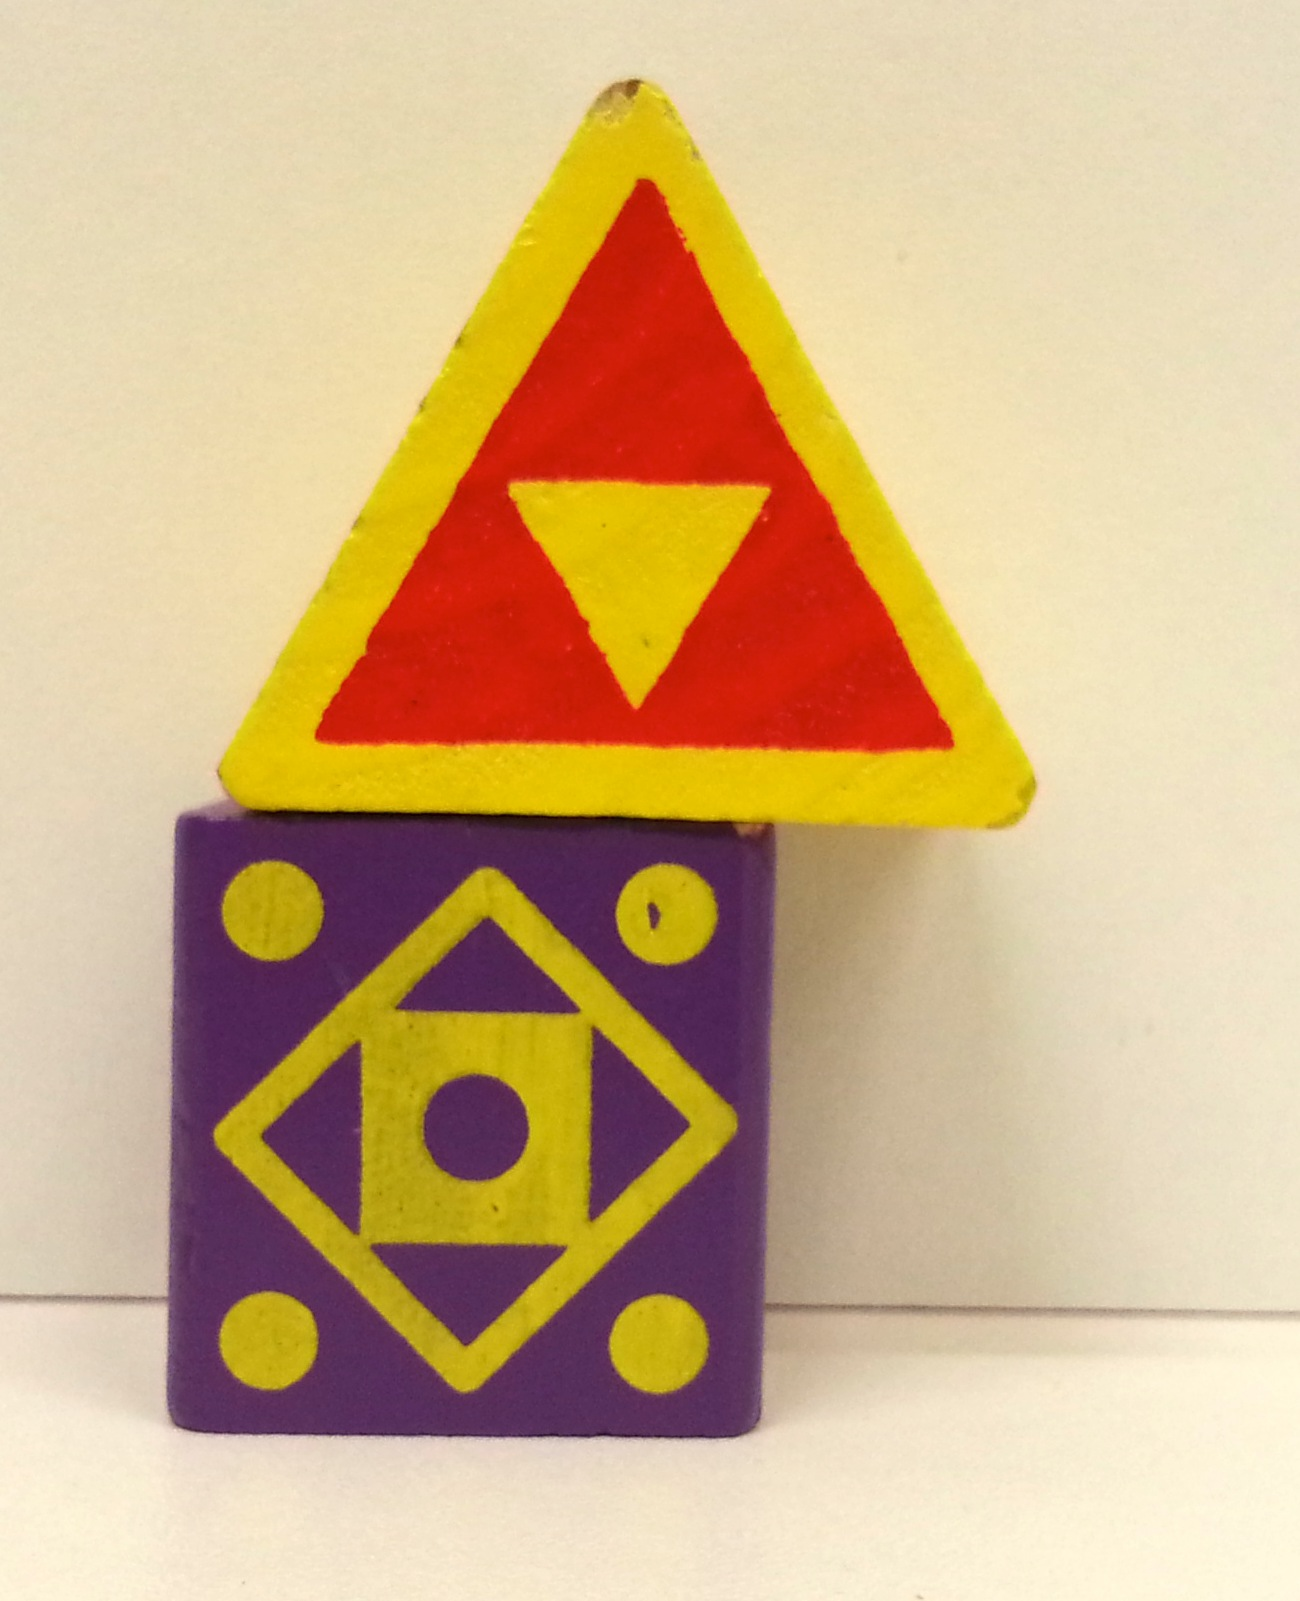
\includegraphics[width=0.3\columnwidth]{PicsforIROS2014/ExamplePositive}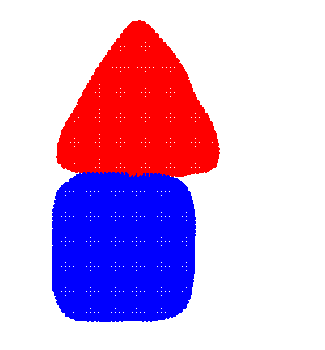
\includegraphics[width=0.3\columnwidth]{PicsforIROS2014/PosExample} & 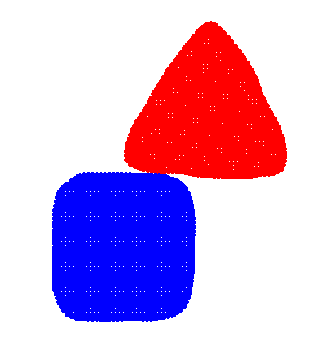
\includegraphics[width=0.3\columnwidth]{PicsforIROS2014/NegExample}\tabularnewline
Positive Example & Negative Example\tabularnewline
\end{tabular}\caption{\label{fig:example-stack-scenes}Point cloud examples of a stable
and an unstable stacking of blocks }
\end{figure}


\subsubsection*{Experimental Setup}

The robot performed $60$ randomly selected grasps along the length of
a spaghetti box. The first half of the grasps were performed with
a three-fingered grasp and the other $30$ were executed with a four-fingered
grasp, as shown in Fig. \ref{fig:Grasp-types}. The robot subsequently
tried to lift the box $13$ cm above the table. The picking up of
the box was considered successful if the object was no longer in contact
with the table, and a failure otherwise, as shown in Fig. \ref{fig:good-and-bad-lift}.
Before lifting the box, the robot recorded the state of the scene
and computed the contact distribution. Based on this information, the robot had to predict whether
or not the lift would be successful. In order to detect contact points,
we labeled ten points in one scene to train the contact classifier.
The contact distribution is defined relative to the center of gravity.

In addition to evaluating the method explained in Section~\ref{sec:Classifying-Object-Interactions},
referred to here as \noun{normal+pos}, we also evaluated several benchmark
approaches. The first benchmark approach, \noun{meanonly,} performs
the classification using only the mean contact $\vec{\mu}_{i}$. The
\noun{pos} approach uses only the position distribution of the contact
points and not the normals. As a result, the contact distribution
is only 3D. Although the fingers do not have tactile sensors, forces
can be roughly approximated using the joint torque sensors of the
fingers and the relative positions of the contact points. The \noun{force+pos
}approach is the same as \noun{normal+pos}, except that the normals
$\vec{u}_{i}$ have been replaced by force estimates. The final method
\noun{handrelative} uses the positions and estimated forces of the
contact points, but defines the contact distribution relative to the
hand rather than the object center. 

The performance of the various methods were tested for different numbers
for training samples. In each evaluation, ten grasps were selected
as test samples. From the remaining grasp samples, a subset of samples
were selected as training data. The classifier was then trained on
the training data and used to classify the test samples. The error
rate is given by the percentage of correctly classified grasps in
the test set. This process was repeated $250$ times for each classifier
and each number of training samples. The results of the evaluation
are shown in Fig. \ref{fig:Lifting-Results}. 

\begin{figure}
\centering{}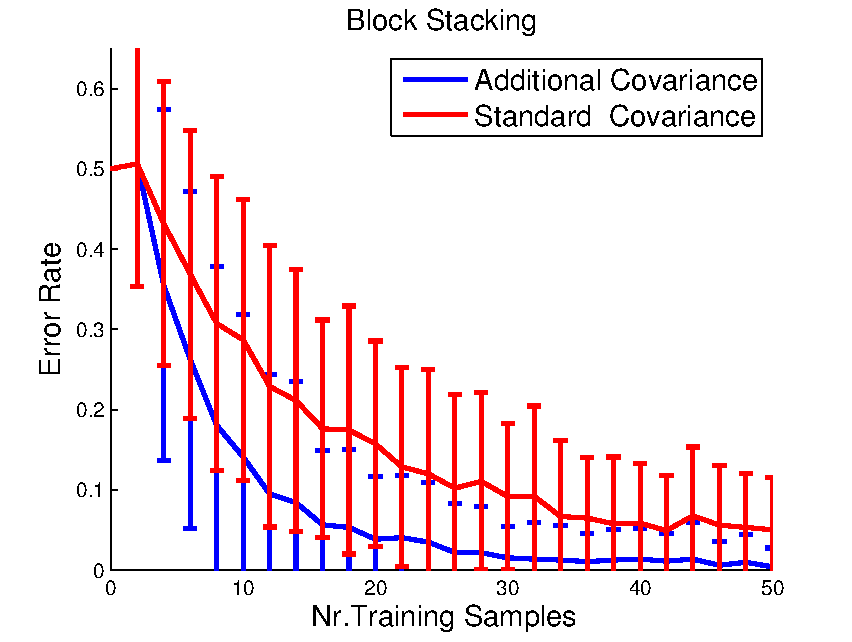
\includegraphics[width=0.94\columnwidth]{PicsforIROS2014/StackingResults2}\caption{\label{fig:stacking result}The expected error rate for the block stacking task. The red line indicates the performance when using the standard covariance matrix. The blue line shows the performance when adding the interaction-specific covariance matrix. The error bars indicate one standard deviation.}
\end{figure}

\subsubsection*{Discussion}

Using only the mean contact or the distribution relative to the hand
resulted in poor performance. The task was especially challenging
for the \noun{handrelative} approach, as the object has the same shape
along its length. Despite this challenge, the approach still obtained
an error rate of $25.04\%$.

Using only the position of the contact points relative to the object
center resulted in an error rate of $18.36\%$, which is only marginally
better than the performance of \noun{handrelative}. In comparison,
the \noun{normal+pos} and the \noun{force+pos} achieved error rates
of $4.88\%$ and $5.28\%$ respectively. The contact normals clearly
capture a considerable amount of information, as they allow side contacts
to be differentiated from top contacts. 

Both\noun{ normal+pos} and \noun{force+pos} performed well on the
task, and learned to accurately predict steady lifts. However, both
approaches also have their limitations. The \noun{normal+pos} approach
cannot differentiate between the robot gently placing its fingers
on the box and the fingers applying forces at the contacts. This approach
can therefore sometimes only predict whether an interaction is possible,
given the contacts, but not if the interaction is being performed.
The \noun{force+pos }approach can differentiate between these two
scenarios, and using it together with tactile sensing is a promising
direction for future research. However, as the forces between objects
will often not be directly observed, the \noun{normal+pos} approach
is generally more applicable. 


\subsection{Stacking Objects}

In the second experiment, the robot was given the task of classifying
whether one object was supporting another. The robot then used the
trained classifier to stack assorted toy blocks.


\subsubsection*{Classifying Stable Block Placements\label{sub:stackingexperiment}}

\begin{figure}
\begin{centering}
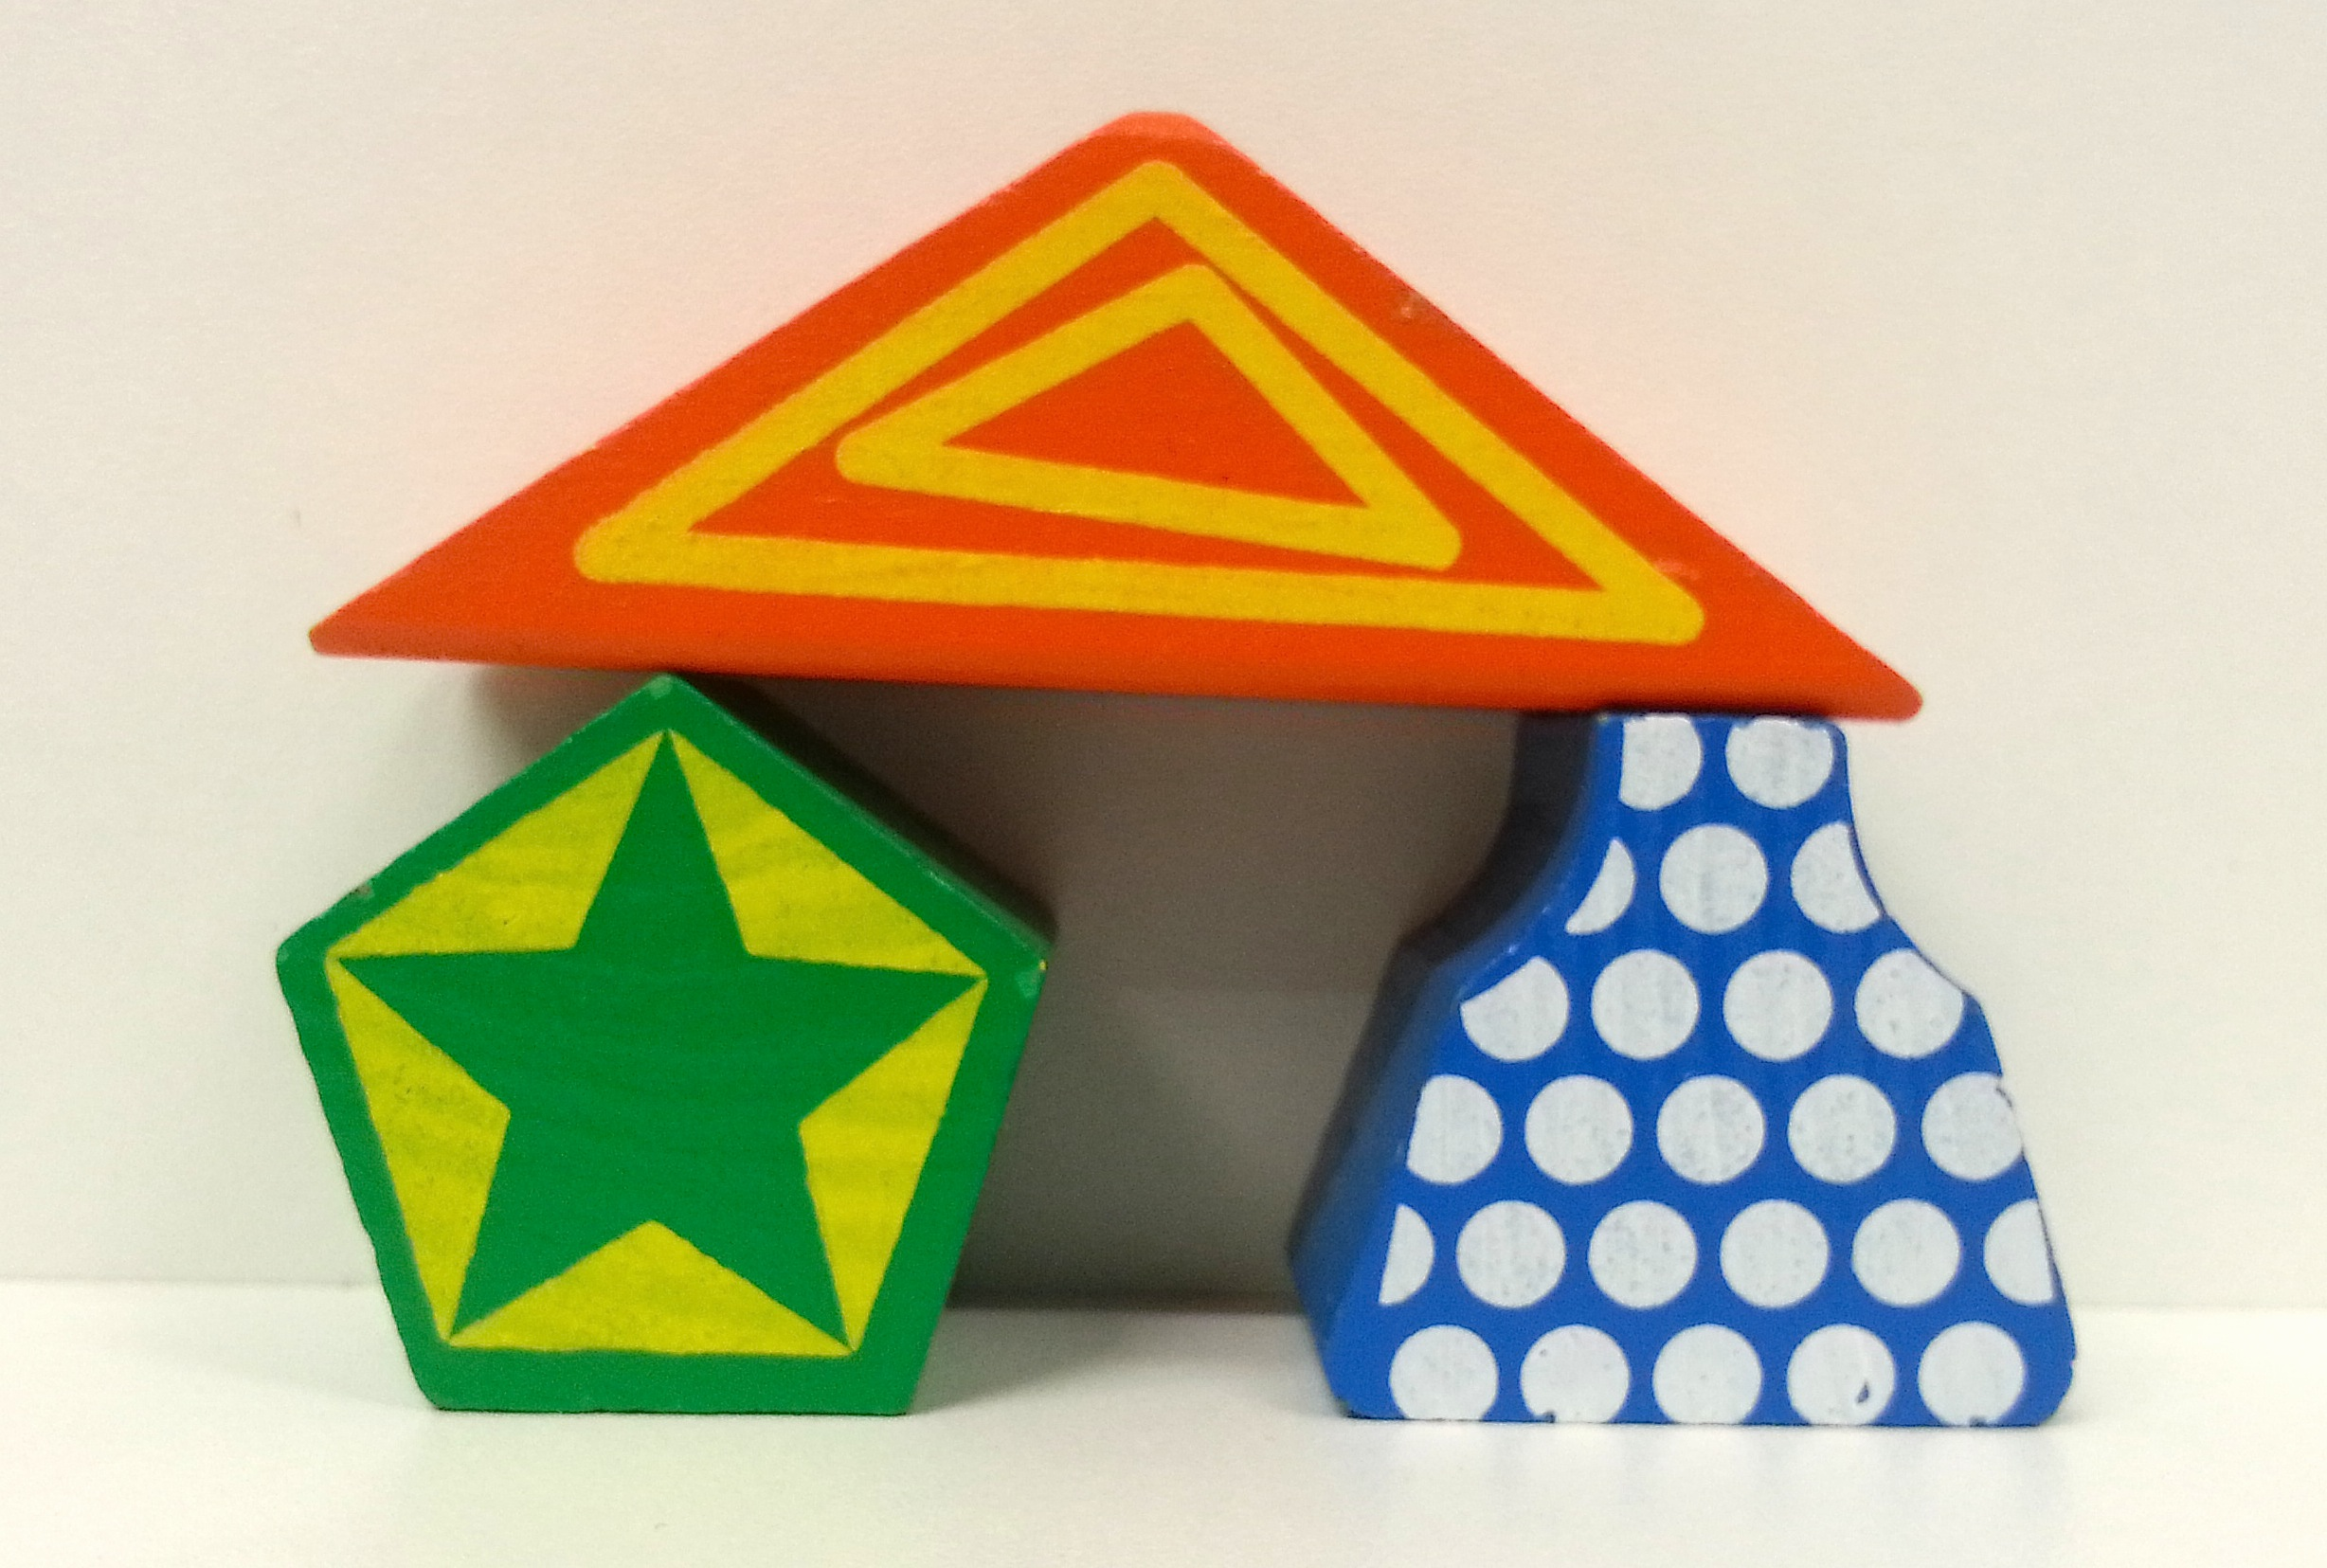
\includegraphics[width=0.5\columnwidth]{PicsforIROS2014/3BlockScene}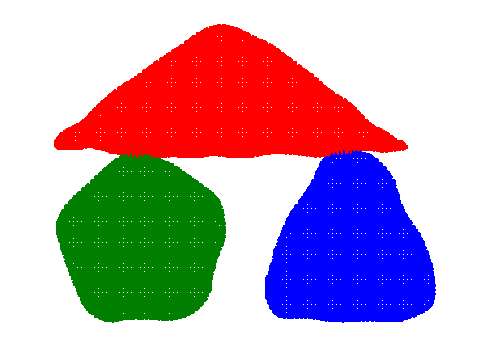
\includegraphics[width=0.5\columnwidth]{PicsforIROS2014/3Blocks}
\par\end{centering}

\caption{\label{fig:3-block-example-scene}An example scene with three objects,
wherein the green and blue objects are supporting the triangular red
block.}
\end{figure}
The robot was provided with $60$ example scenes, each containing two
interacting toy blocks, such as the ones shown in Fig. \ref{fig:example-stack-scenes}.
For the $30$ negative examples, physically impossible static scenes
were created by hand. The models of the blocks were acquired using
a turn table setup and a kinect. The object center is again defined
by the center of gravity. To train the contact point classifier, ten
points were hand labelled in one scene. The points of the object were
classified as contacts based on the features described in Section
\ref{sub:Contact-Points}. Using additional features, such as the
position and orientation of the points relative to the object's center,
were also tested, but had no significant effects on the outcome of
the experiment. 

The performance of the contact point classifier was evaluated in the
same manner as for the previous experiments. A set of ten test samples
were randomly selected and removed from the pool of $60$ samples. A
subset of the remaining samples were then used to train the classifier.
The classifier was subsequently applied to the ten test samples, and
the error rate was recorded. The error rate is $1$ if all ten samples
were incorrectly classified, and $0$ if all of them were correctly
classified. The test samples were subsequently put back into the pool
of samples. This process was repeated $250$ times for each number of
training samples. 

In addition to the standard approach, we also evaluated adding an
interaction-specific covariance matrix $\tilde{\vec{\Sigma}}$, as
explained in Section \ref{sub:interspecvar}. The elements of the diagonal matrix were
recomputed for each trial using a basic hill-climbing approach to minimize
the leave-one-out cross-validation error rate on the training set.

The results of this experiment are shown in Fig. \ref{fig:stacking result}.
Starting with error rates close to $50\%$, the classifiers' performances
gradually improves as more samples are provided. Given $50$ samples,
the standard classifier achieved an expected error rate of $5.0\%$,
and could accurately predict when the object was being supported. Using
the additional interaction-specific covariance matrix, the classifier
achieved an expected error rate of $0.4\%$ for $50$ samples, and
only required $20$ samples to achieve an expected error rate of $3.84\%$.
The sample efficiency of the algorithm can therefore be increased
by incorporating the interaction-specific covariance.
In many of the trials, the covariance matrix $\tilde{\vec{\Sigma}}$ indicated that
the vertical position of the supporting contacts was less relevant
than the horizontal position. The experiment
demonstrates the classifier's ability to generalize between different
object shapes. 



\subsubsection*{Generalization to Multiple Objects}

In order to demonstrate the classifier's ability to generalize to
multiple objects, it was applied to the scene of three objects shown
in Fig. \ref{fig:3-block-example-scene}. In this scene, the top object
is being supported by both of the lower objects. When the classifier
is applied to the top block and only one of the bottom blocks, the
interaction is classified as not supporting. However, we can also
combine the blue and green point clouds of the bottom objects in order
to create one compound object. When applying the classifier to the
top object and this compound object, the top object is labeled as
being supported by the bottom object. Thus, as one would expect, the
classifier detects that the top is being supported by both objects
jointly, and by neither one separately. The classifier was tested
on two more similar scenes of three blocks, with the same results.


\subsubsection*{Building Block Towers}

\begin{figure}
\begin{centering}
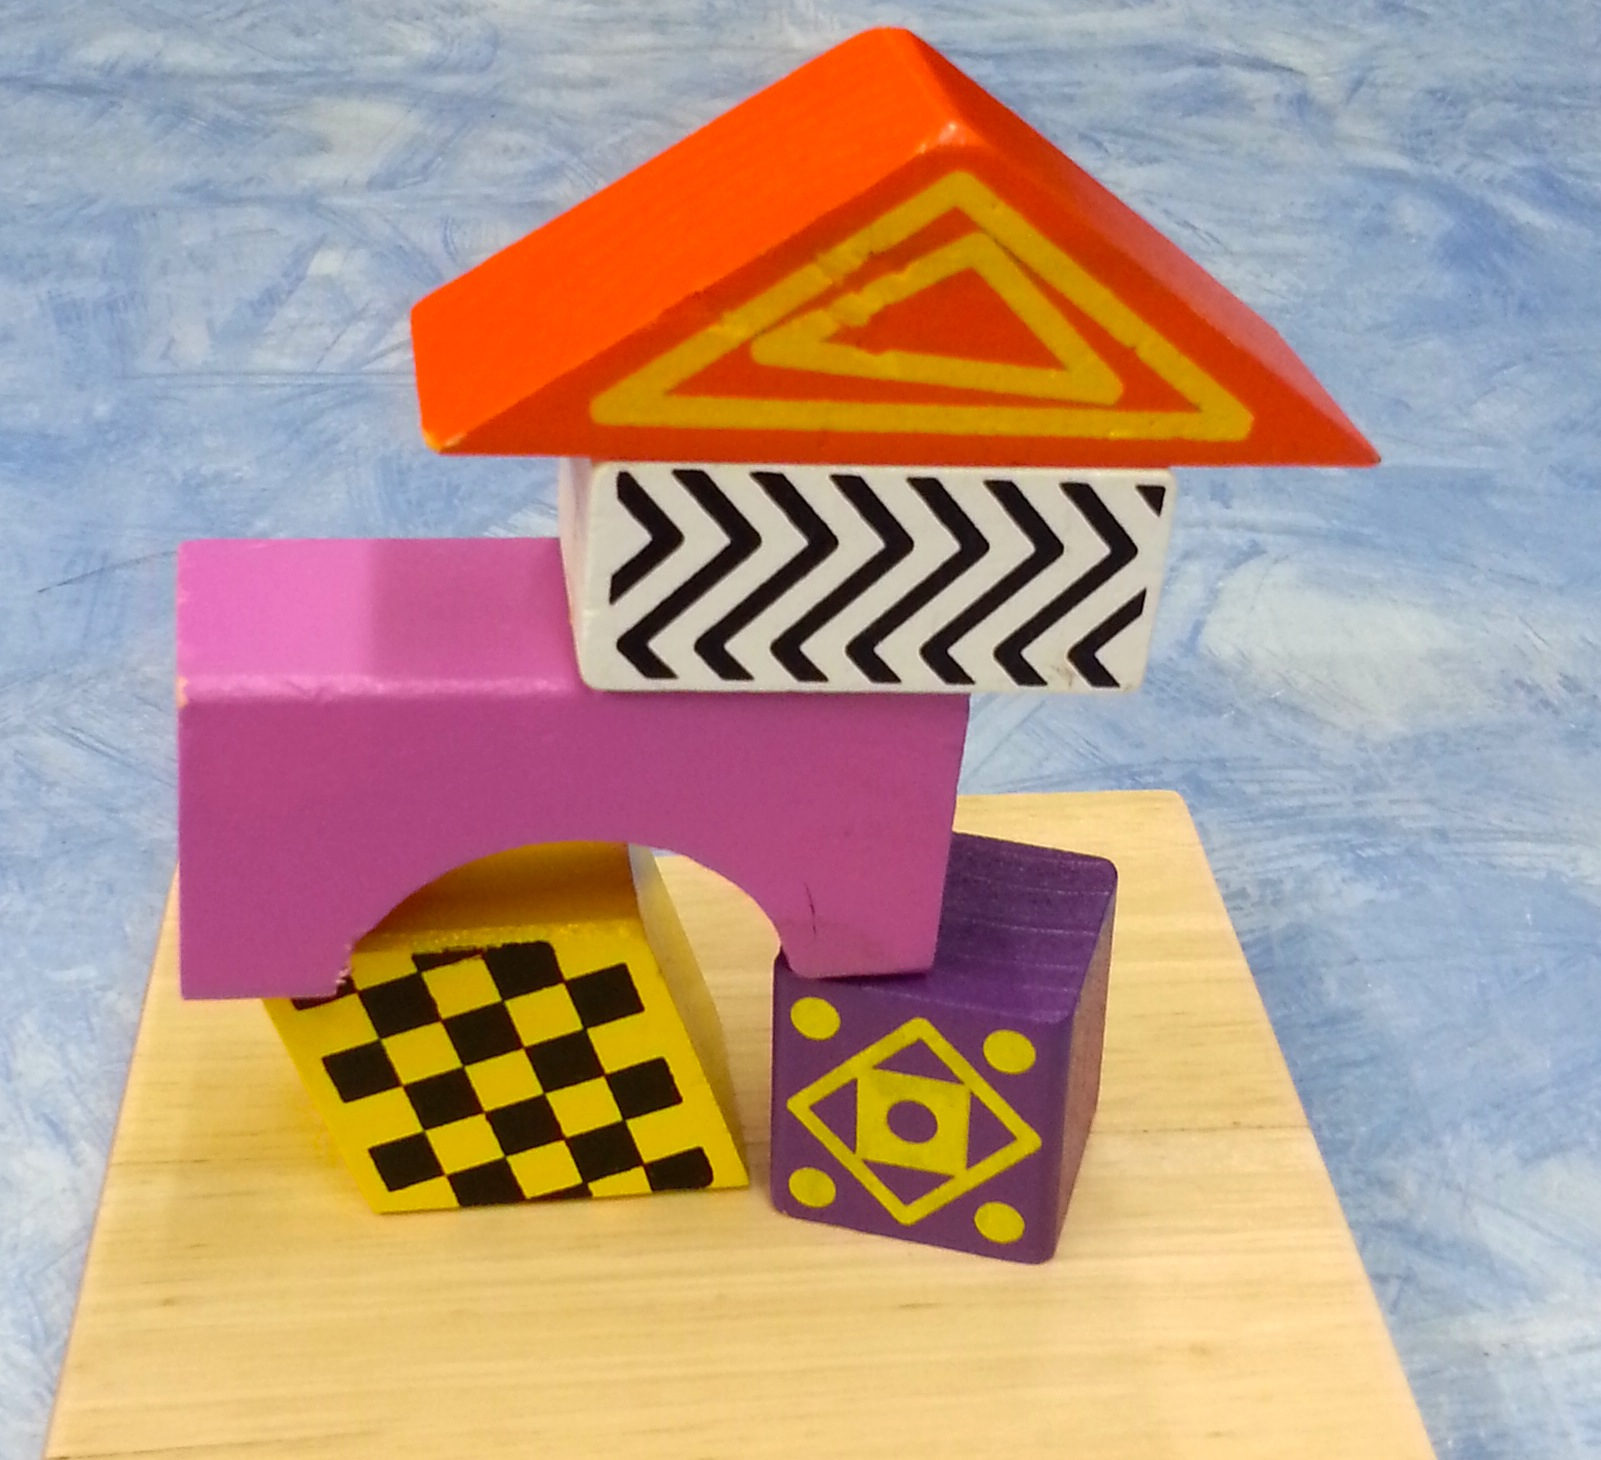
\includegraphics[width=0.49\columnwidth]{/Users/oliver/Documents/Publications/IROS2014/PicsforIROS2014/Pile1}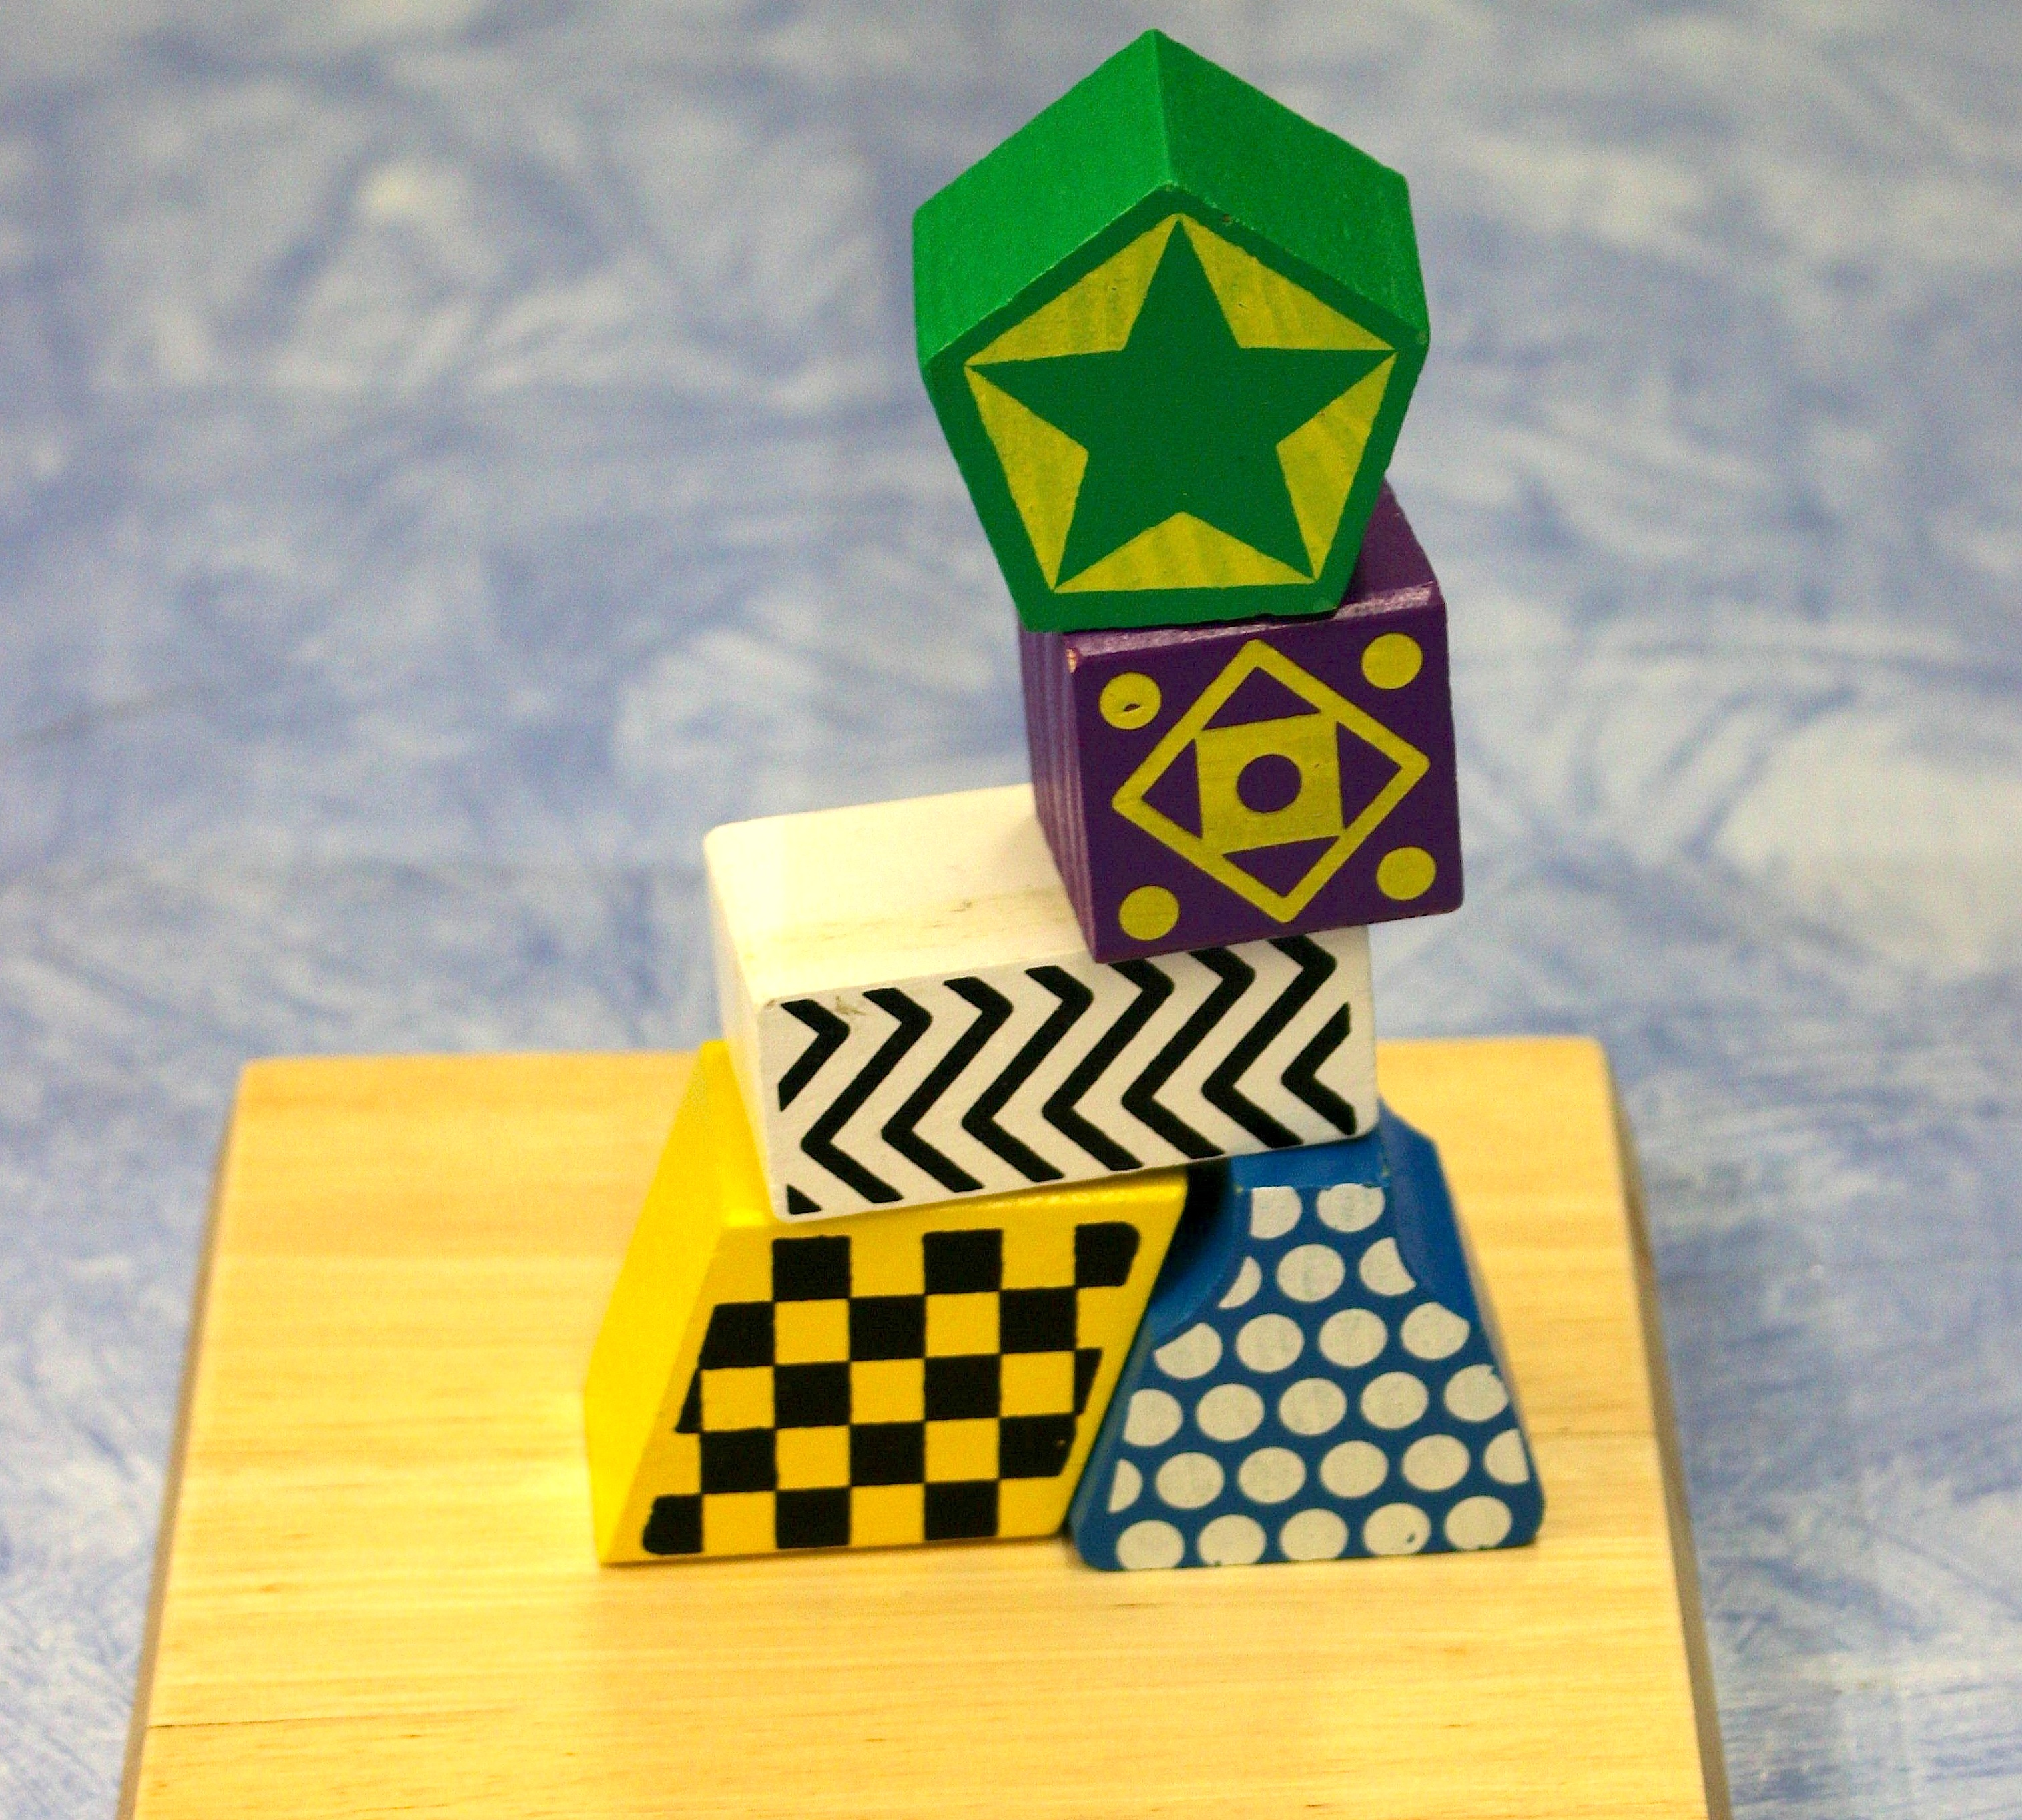
\includegraphics[width=0.4965\columnwidth]{/Users/oliver/Documents/Publications/IROS2014/PicsforIROS2014/Pile2}
\par\end{centering}

\caption{\label{fig:blocktowers}Two examples of block towers constructed by
the robot.}
\end{figure}
In the final part of the experiment, the real robot used the classifier
from the first part to perform block stacking. The interaction-specific
covariance matrix was not used in this experiment. The robot was provided
with a small wooden board, on which to stack the blocks. In order
to avoid all of the blocks being placed directly on the board, the
placing of the blocks was limited to a single strip along the middle
of the board. For every block, the robot observed the current scene
using the kinect and used the resulting point cloud as the supporting
object in the interaction. As the focus is not on the planning aspects
of the problem, the sequence of blocks was predefined. 

In order to determine a suitable placement for the current block, the robot sampled different
positions in the scene. For each sample, the contact points were estimated
and the probability of the block being supported was computed. The
robot then attempted to place the block at the position with the highest
probability. 

Randomly sampling positions in the scene led to poor performance.
One of the main challenges for the robot was the noisy partial point cloud
of the current scene. The kinect usually only captured the top and
front of the current block stack, but not the back or sides. The lack
of reliable points on the sides of objects resulted in unforeseen
collisions between blocks. This problem could be alleviated by obtaining
more views of the scene, completing the point cloud based on symmetries
\cite{BohgMindtheGap,Kroemer_Humanoids_2012}, or applying a penalty for
placing the block into occluded regions. 

In order to reduce the number of accidental collisions, we also implemented
a sampling approach that mimics the movement of the block when it is being put down. 
The robot sampled $20$ horizontal positions at $7.5$mm 
increments across the width of the board. For each horizontal position, the robot sampled
vertical placements at $5$mm increments in a top-down manner until
contact was detected between the block and the stack. 

In order to evaluate the proposed approach, the robot was given 
the task of creating five towers consisting of five blocks each. 
Using the improved sampling approach, the robot
successfully placed $96\%$ of the blocks without knocking any blocks down. 
Only one block was  misplaced by a few millimeters and fell down. The robustness of
the system could be further improved by  also considering the probability of 
success of neighboring positions \cite{Boularias2011}.  

The robot currently ignores the interactions between blocks further down 
in the stack. As a result the robot may select
a block placement that causes a supporting block to fall down. One potential
solution to this problem would be to recheck the interactions between
objects further down the stack. For each interaction, the objects
higher up in the stack would then be treated as a single compound
object, with a corresponding object center. This approach would however
require the robot to keep a model of the current scene's geometry. 

 The results of the experiment show that the robot was able to construct multiple
block towers, such as the ones shown in Fig. \ref{fig:blocktowers},using the proposed approach.
A video of the robot stacking blocks is avaliable at: http://youtu.be/6S5eJgE28sg


\section{Conclusions}

In this paper, we presented a kernel-based approach to learning
object interactions from contact distributions. The proposed approach
is based on modeling the distribution of contact points as a Gaussian
distribution. The Bhattacharyya kernel is then used to compute
the similarity between the contact distributions. In the experiments,
we used kernel logistic regression to predict stable grasps of objects,
as well as suitable placements of objects. Using the learned classifier,
the robot was able to build small towers out of assorted blocks. 


\section{Acknowledgments}

The research leading to these results has received funding from the
European Community's Seventh Framework Programme 
under grant agreements 610878 (3rdHand), 600716 (CoDyCo), and 610967 (TACMAN).

\bibliographystyle{plain}
\bibliography{ContactBib}

\end{document}
